Neste capítulo, abordamos a análise de sentimento como uma ferramenta poderosa no contexto do processamento de linguagem natural, focando especialmente nas postagens do Colab. Exploramos como técnicas de aprendizado de máquina, particularmente com o uso do Natural Language Toolkit (NLTK), podem ser empregadas para automatizar e aprimorar a análise de sentimentos. Além disso, discutimos a relevância de identificar diferentes "personas" de usuários, como os \textit{helpers} e \textit{complainers}, e como essa distinção pode influenciar a dinâmica e a polarização dentro de uma plataforma de mídia social. Finalmente, abordamos a relação entre análise de sentimento, polarização e a formação de câmaras de eco, destacando a importância de entender e mitigar esses fenômenos em ambientes digitais.

\section{Análise exploratória de Sentimento}

Neste capítulo, nos aprofundamos na análise de sentimentos das postagens do Colab, introduzindo a métrica de "score". Esta métrica foi desenvolvida especificamente para este estudo, com o intuito de classificar as postagens como positivas ou negativas, proporcionando uma visão mais quantitativa dos sentimentos expressos pelos usuários. Além disso, apresentamos uma análise exploratória dos dados, com o objetivo de identificar os principais tópicos discutidos no Colab e as principais palavras associadas a cada tópico. Por fim, adicionamos uma camada de análise de redes no experimento, introduzindo a assortatividade como uma métrica para medir a homofilia na rede.

Para realizar essa análise, fundamentamos nosso estudo em conceitos e técnicas de processamento de linguagem natural (PLN) e análise de sentimentwos. O PLN é uma área da inteligência artificial que visa capacitar os computadores a entender, interpretar e gerar linguagem humana de forma natural. A análise de sentimentos, por sua vez, é uma subárea do PLN que se concentra em identificar e extrair informações sobre os sentimentos e opiniões expressos em textos.

Utilizamos a linguagem de programação Python como base para a implementação do experimento. Como runtime, novamente utilizamos o Google Colab, que nos permite executar o código em nuvem, sem a necessidade de instalar bibliotecas ou configurar o ambiente de desenvolvimento. O código-fonte do experimento está disponível no GitHub\footnote{https://github.com/guinetik/colab-network-ec}.

Com a aplicação dessas técnicas e o uso da linguagem Python, pudemos extrair insights valiosos sobre os sentimentos presentes nas postagens do Colab. Essas métricas servirão como base para as análises subsequentes e contribuirão para aprimorar a compreensão do ecossistema do Colab.

\subsection{Heurísticas para classificação de postagens por score de sentimento}

No capítulo anterior, realizamos uma análise exploratória da rede, identificando comunidades de usuários e suas interações. Neste contexto, a classificação de postagens por score torna-se uma ferramenta valiosa. Esta métrica categoriza as postagens como positivas, negativas ou neutras com base em seu conteúdo textual, utilizando uma abordagem de pontuação de sentimentos. Cada postagem recebe um score de sentimento que varia de -1 (negativo) a 1 (positivo), com scores próximos a 0 indicando neutralidade. Esta abordagem quantitativa não só nos permite capturar o sentimento geral expresso nas postagens, mas também entender como esses sentimentos se propagam e interagem dentro da rede. Assim, podemos obter insights valiosos sobre a percepção dos usuários em relação a diferentes tópicos e como essa percepção influencia a estrutura e a dinâmica da rede.

O processo de análise de sentimento das postagens começa com o carregamento dos dados. Nessa análise, estamos interessados em postagens criadas por usuários das comunidades identificadas na análise do capítulo anterior, nas cidades de Niterói, Santo André e Mesquita. Em seguida, realizamos o pré-processamento do texto, que envolve a remoção de caracteres especiais, conversão para letras minúsculas, tokenização e aplicação de técnicas de stemização para reduzir as palavras às suas formas básicas \cite[]{2009_Bird_BOOK}.

Utilizamos a técnica de "bag-of-words" descrita em \citeonline{2013_Mikolov} com a biblioteca CountVectorizer para converter o texto em uma matriz numérica, onde cada coluna representa uma palavra e cada linha representa uma postagem. Com base nessa matriz, identificamos as palavras mais frequentes e as visualizamos em um gráfico de barras e na forma de uma nuvem de palavras.

\begin{quadro}[!htb]
	\caption{Distribuição de palavras mais frequentes}
	\label{fig:wordcount}
	\centering
	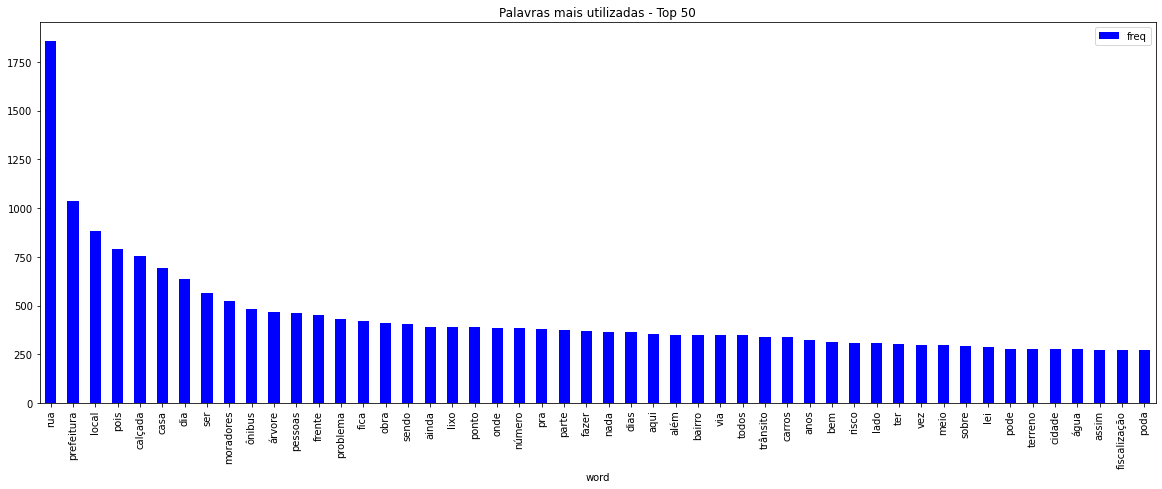
\includegraphics[width=\textwidth]{images/wordcount.png}
	\fautor
\end{quadro}

Realizamos uma análise exploratória dos dados para entender melhor as características das postagens. Isso incluiu a visualização da distribuição das palavras mais frequentes e a criação de nuvens de palavras para postagens positivas e negativas. Além disso, utilizamos a biblioteca Word2Vec para criar um modelo de palavras em vetores, que foi usado para visualizar as associações de palavras mais comuns.

\begin{figure}[!htb]
	\caption{Núvem de palavras mais utilizadas}
	\label{fig:wordcloud}
	\centering
	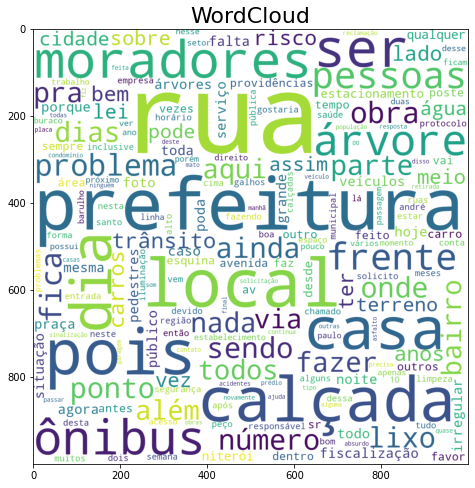
\includegraphics[scale=0.5]{images/wordcloud.png}
	\fautor
\end{figure}

\begin{figure}[htb]
	\centering
	\caption{Comparação de núvem de palavras mais usadas}\label{fig:lexicon_tagcloud}
	\begin{subfigure}[b]{0.317\textwidth}
		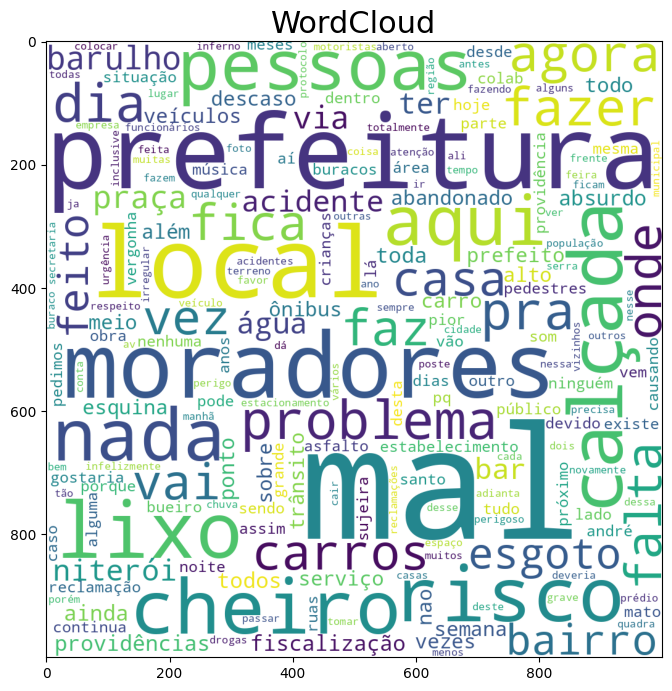
\includegraphics[width=\textwidth]{images/lexicon_worst_scores_tagcloud.png}
		\caption{Scores Negativos}
		\label{fig:tigre}
	\end{subfigure} ~ %add desired spacing between images, e. g. ~, \quad, \qquad, \hfill etc. %(or a blank line to force the subfigure onto a new line) 
	\begin{subfigure}[b]{0.317\textwidth}
		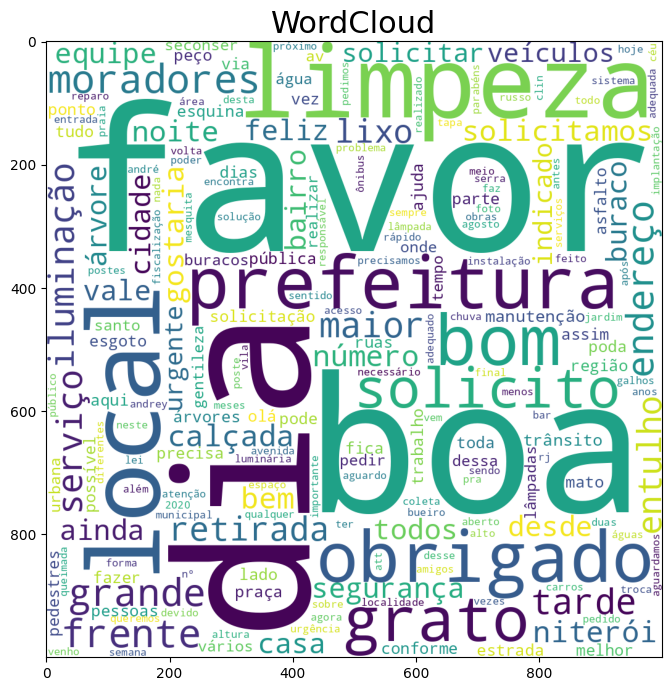
\includegraphics[width=\textwidth]{images/lexicon_best_scores_tagcloud.png}
		\caption{Scores Positivos} \label{fig:leao}
	\end{subfigure} ~ %add desired spacing between images, e. g. ~, \quad, \qquad, \hfill etc. %(or a blank line to force the subfigure onto a new line)
	\fautor
\end{figure}

\section{Análise das postagens em Niterói, Santo André e Mesquita}

\begin{quadro}[!htb]
	\caption{Distribuição dos scores de sentimento nas postagens da rede das 3 cidades selecionadas. Cada ponto representa um usuário e a cor indica o score médio de sentimento de suas postagens (verde para positivo, vermelho para negativo e laranja para neutro)}
	\label{fig:scores_scatterplot}
	\centering
	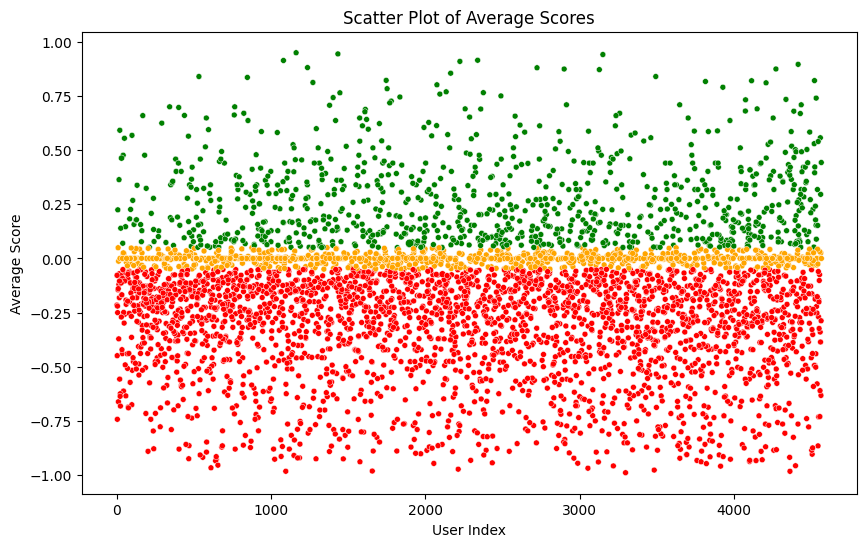
\includegraphics[scale=0.70]{images/scores_scatterplot.png}
	\fautor
\end{quadro}

Após a seleção das postagens dos usuários das comunidades das cidades de Niterói, Santo André e Mesquita, conforme detalhado no capítulo anterior, foi possível identificar um total de 132.846 eventos de zeladoria criados por membros dessas comunidades. Esta vasta quantidade de dados nos ofereceu uma oportunidade única para aprofundar nossa análise de sentimentos e entender melhor as emoções e opiniões expressas pelos usuários.

Ao aplicar a análise de sentimentos nas postagens, foi essencial considerar a extensão dos textos. Uma postagem mais longa tem naturalmente mais palavras e, consequentemente, uma maior soma de polaridades. Para contornar essa característica e garantir uma análise justa, optamos por normalizar os scores com base no número de tokens ou palavras presentes na frase original. Esta abordagem permitiu que cada palavra contribuísse proporcionalmente para o score final da postagem, independentemente do seu tamanho.

Ao examinar os melhores scores, notamos algumas tendências interessantes. Primeiramente, as postagens com os scores mais elevados tendem a ter uma combinação de sentimentos neutros e positivos, conforme indicado pelas métricas do LeIA. Por exemplo, a postagem do evento 100876, originada de Niterói, apresenta uma combinação de 75,1\% de conteúdo neutro e 16,8\% de conteúdo positivo, resultando em um score composto de 0,671. Isso sugere que, mesmo quando os usuários estão apresentando informações factuais ou descritivas, há uma inclinação positiva em suas expressões.

Além disso, é notável que, mesmo com variações nos scores derivados dos dicionários léxicos, o LeIA consistentemente percebeu essas postagens como altamente positivas. Isso pode ser atribuído à capacidade do LeIA de capturar nuances e contextos específicos da língua portuguesa, como a influência de emojis e a presença de negações.

Outro ponto de destaque é a variedade de temas abordados nas postagens com os melhores scores. Enquanto algumas postagens focam em questões de zeladoria como o acúmulo de lixo, outras discutem colaborações entre organizações privadas e públicas. Isso reforça a ideia de que a plataforma Colab é um espaço diversificado, onde os usuários se sentem empoderados para discutir uma ampla gama de tópicos relacionados à melhoria de suas comunidades.

Em resumo, a análise dos melhores scores nos proporcionou uma visão mais clara das emoções e opiniões dos usuários nas comunidades selecionadas. Estes insights são fundamentais para entender as motivações dos usuários ao interagir na plataforma e podem ser usados para orientar futuras estratégias de engajamento e moderação.

\begin{quadro}[!htb]
	\caption{Score médio de sentimento por número de usuários}
	\label{fig:average_score_by_number_of_users}
	\centering
	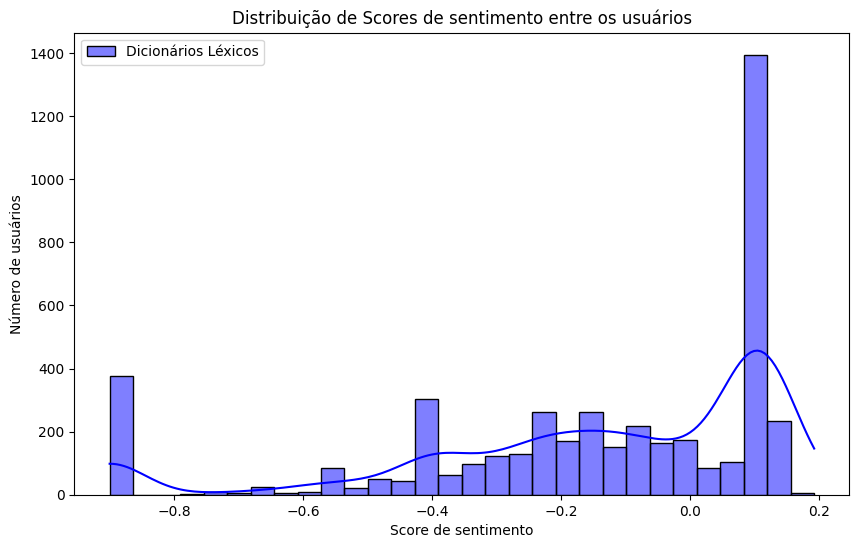
\includegraphics[scale=0.70]{images/average_score_by_number_of_users.png}
	\fautor
\end{quadro}

Ao analisar os piores scores, é evidente que as postagens refletem um alto grau de insatisfação e frustração dos usuários em relação a questões específicas de zeladoria em suas comunidades. Estas postagens, oriundas das cidades de Niterói e Rio de Janeiro, destacam-se não apenas pelo conteúdo negativo, mas também pela intensidade das emoções expressas.

A postagem do evento 218258, por exemplo, menciona a repetição de reclamações feitas pelo usuário sem a devida solução, indicando um sentimento de desamparo e descontentamento com a resposta (ou falta dela) das autoridades competentes. O score derivado do dicionário léxico para esta postagem foi de -2.857, enquanto o LeIA identificou uma predominância de conteúdo neutro (73,5\%), mas com uma porcentagem significativa de conteúdo negativo (19,9\%). O score composto, que combina ambas as métricas, resultou em -0.957, refletindo a natureza altamente negativa da postagem.

Da mesma forma, a postagem do evento 156161 expressa indignação com a situação de uma rua específica, usando palavras em caixa alta para enfatizar o descontentamento. O uso de termos como "ABSURDO" e "CAOS" sugere uma forte emoção negativa. O LeIA capturou essa nuance, atribuindo um score negativo de -0.9930, enquanto o score do dicionário léxico foi de -0.167. A combinação de ambos resultou em um score composto de -0.956.

É interessante notar que, mesmo nas postagens com os piores scores, ainda há uma presença de conteúdo neutro e, em alguns casos, até mesmo positivo. Por exemplo, a postagem do evento 239454, apesar de expressar frustração com tentativas repetidas de comunicação, ainda contém uma saudação cordial ("Olá prezados"). Isso sugere que, mesmo em meio à insatisfação, os usuários ainda buscam manter um tom respeitoso e construtivo em suas comunicações.

Em resumo, as postagens com os piores scores ilustram claramente os desafios e frustrações enfrentados pelos usuários em suas comunidades. Estas postagens são valiosas, pois destacam áreas que requerem atenção imediata e melhorias por parte das autoridades locais. Além disso, a análise de sentimentos fornece uma ferramenta poderosa para identificar e compreender essas preocupações, permitindo uma resposta mais eficaz e empática por parte dos tomadores de decisão.

\begin{quadro}[!htb]
	\caption{Distribuição de quantidade de postagens por score}
	\label{fig:score_distribution}
	\centering
	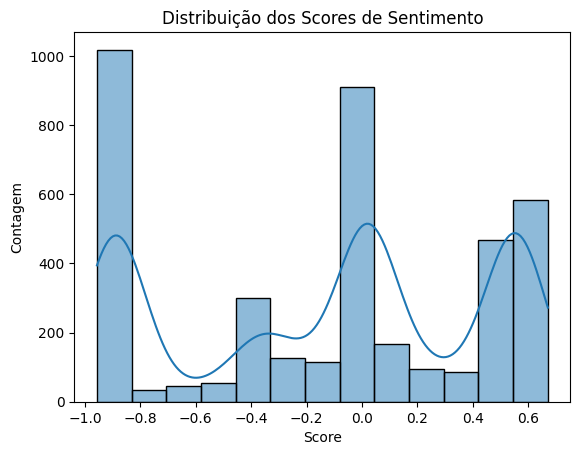
\includegraphics[scale=0.90]{images/score_distribution.png}
	\fautor
\end{quadro}

Após obter o score de sentimento de cada postagem, o próximo passo foi agregar as postagens de cada usuário. Ao calcular a média ponderada do score de sentimento pelo número de postagens, conseguimos criar um score geral que reflete o sentimento médio de todas as postagens de um usuário. Esta métrica agregada nos forneceu uma visão mais clara do panorama geral dos sentimentos expressos nas redes de Niterói, Santo André e Mesquita.

\begin{figure}[htbp]
	\centering
	\begin{subfigure}{0.45\textwidth}
		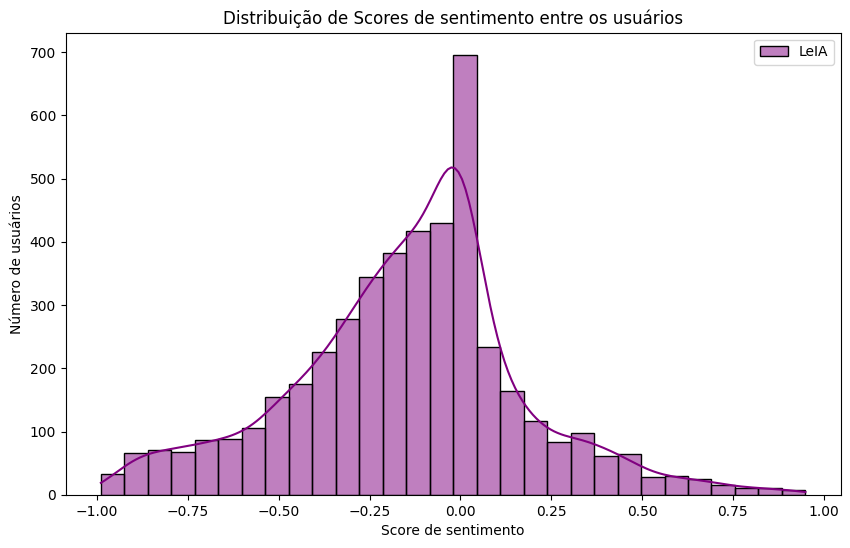
\includegraphics[width=\linewidth]{images/average_leia_by_number_of_users.png}
		\caption{Score Composto LeIA}
		\label{fig:average_leia_by_number_of_users}
	\end{subfigure}
	\hfill
	\begin{subfigure}{0.45\textwidth}
		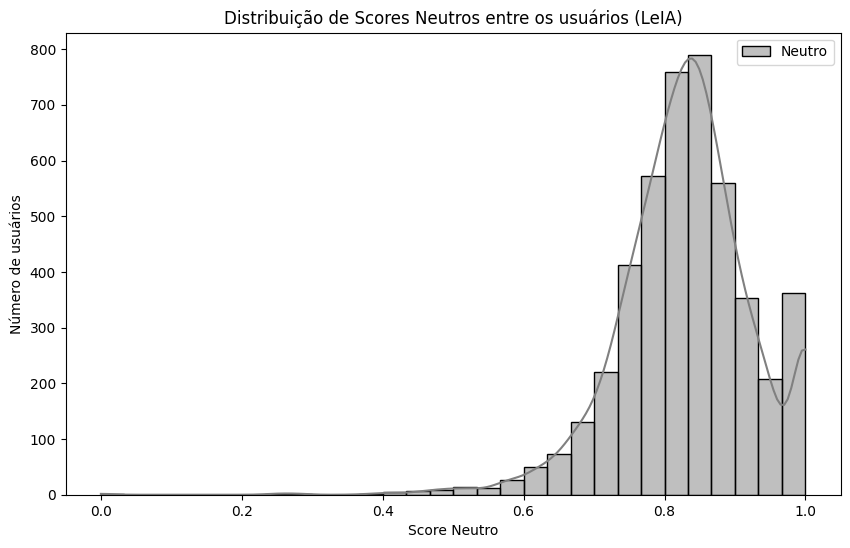
\includegraphics[width=\linewidth]{images/average_neutral_by_number_of_users.png}
		\caption{Neutros}
		\label{fig:average_neutral_by_number_of_users}
	\end{subfigure}
	\vskip\baselineskip
	\begin{subfigure}{0.45\textwidth}
		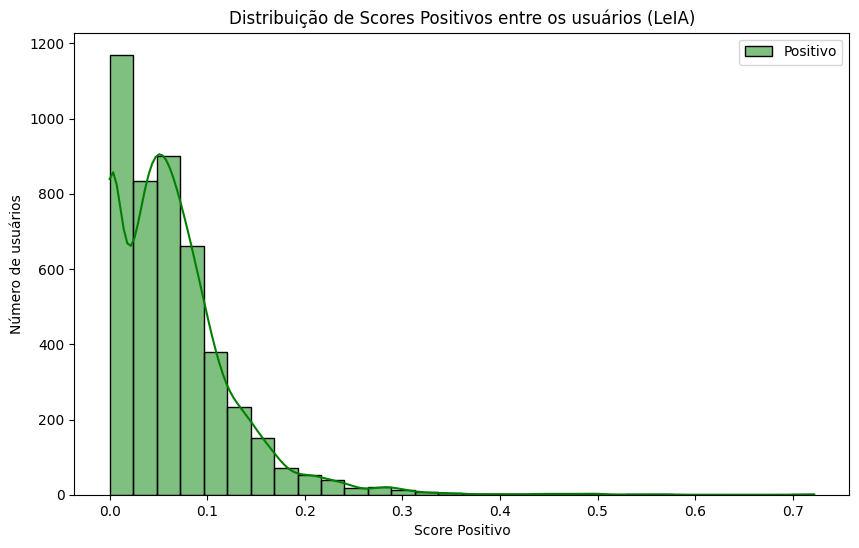
\includegraphics[width=\linewidth]{images/average_positive_by_number_of_users.png}
		\caption{Positivos}
		\label{fig:imagem3}
	\end{subfigure}
	\hfill
	\begin{subfigure}{0.45\textwidth}
		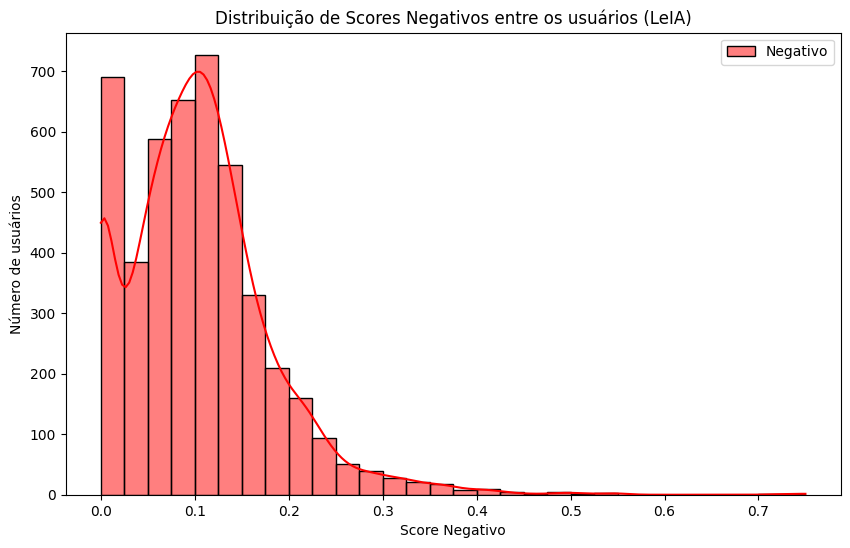
\includegraphics[width=\linewidth]{images/average_negative_by_number_of_users.png}
		\caption{Negativos}
		\label{fig:average_negative_by_number_of_users}
	\end{subfigure}
	\caption{Distribuição dos sentimentos médios em relação ao número de usuários. Os gráficos apresentam uma análise detalhada dos sentimentos, incluindo o score composto pelo LeIA, bem como as categorias neutras, positivas e negativas.}
	\label{fig:average_sentiment_by_number_of_users}
\end{figure}

Com os scores de sentimentos devidamente ajustados, partimos para uma análise mais detalhada dos dados. Uma observação inicial revelou que, ao contrário da premissa inicial de que a maioria das postagens tinha um tom negativo, a distribuição de sentimentos, quando consideramos cada postagem individualmente, mostra que 55.9\% das postagens são positivas, 24\% são negativas e 20.2\% são neutras. No entanto, quando agregamos todas as postagens de um único usuário, observamos que cerca de 67.3\% dos usuários têm postagens majoritariamente positivas, 17.7\% são majoritariamente negativas e 15\% são neutras.

Isso sugere que, embora possa haver uma percepção predominante de que os usuários expressam insatisfação ou preocupações em suas postagens, a realidade é mais matizada. A maioria dos usuários, de fato, tende a compartilhar feedbacks ou observações positivas sobre suas comunidades. Isso pode ser um reflexo de uma série de fatores: talvez os usuários estejam mais inclinados a compartilhar experiências positivas para promover a coesão comunitária, ou talvez as plataformas de mídia social, como o Colab, estejam se tornando espaços onde as pessoas desejam destacar o que está funcionando bem, em vez de apenas apontar problemas.

No entanto, os 24\% de postagens negativas não devem ser negligenciados. Mesmo que representem uma minoria em relação às postagens positivas, elas são cruciais para entender as áreas de preocupação e insatisfação dos usuários. Essas postagens podem ser extremamente valiosas para os tomadores de decisão, pois fornecem insights diretos sobre onde as intervenções podem ser mais necessárias.

As postagens neutras, que compõem 20.2\% do total, também são intrigantes. Elas podem representar uma variedade de conteúdos, desde solicitações de informação até comentários que não expressam uma opinião clara em uma direção ou outra. Essas postagens podem servir como um lembrete de que nem todo feedback pode ser facilmente categorizado como positivo ou negativo, e que a neutralidade em si pode oferecer insights sobre as áreas onde os sentimentos dos usuários são mistos ou incertos.

\begin{quadro}[!htb]
	\caption{Scores de sentimento por quantidade de postagens}
	\label{fig:pie_sentiment_breakdown}
	\centering
	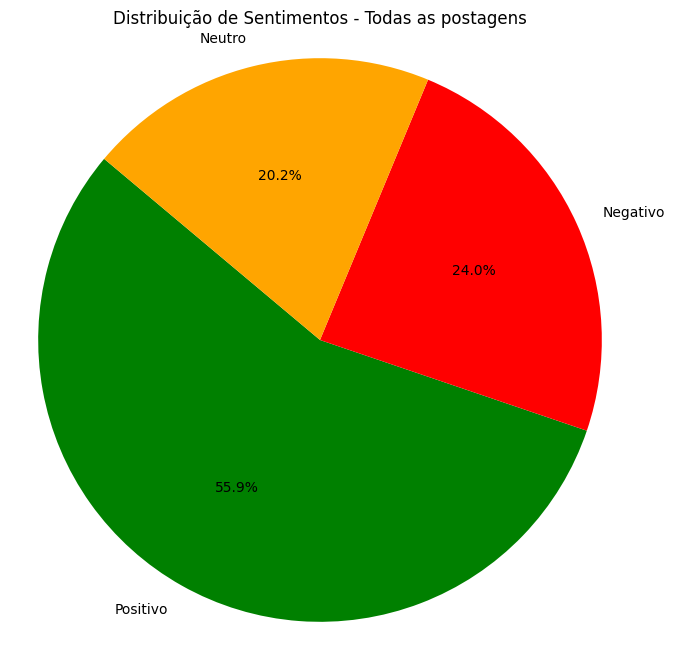
\includegraphics[scale=0.5]{images/pie_sentiment_breakdown.png}
	\fautor
\end{quadro}

Ao analisar os eventos postados, observamos que "Entulho na calçada/via pública" é um dos tópicos mais frequentemente mencionados, com um total de 44.273 postagens. No entanto, é interessante notar que a maioria dessas postagens é classificada como neutra, com 35.391 postagens, seguida por 5.712 postagens positivas e 3.170 postagens negativas. Isso sugere que, embora haja uma alta incidência de relatos sobre entulho nas vias, muitos usuários não expressam uma opinião fortemente positiva ou negativa sobre o assunto.

Outro evento que se destaca é "Lâmpada apagada à noite", com um total de 8.701 postagens. Deste total, 3.212 postagens foram classificadas como neutras, 2.296 como positivas e 3.193 como negativas. Isso indica que há uma divisão nas opiniões dos usuários sobre a questão da iluminação pública à noite, com muitos reconhecendo os esforços para resolver o problema, mas também uma quantidade significativa de postagens expressando insatisfação.

Por outro lado, "Ponto de travessia irregular" teve um total de 46 postagens, das quais 31 foram classificadas como negativas, 6 como neutras e 6 como positivas. Isso sugere que há uma preocupação predominante com a segurança dos pontos de travessia, e que muitos usuários veem isso como uma área que precisa de melhorias.

Em resumo, os dados refletem as preocupações dos cidadãos em relação a diferentes aspectos da infraestrutura e serviços públicos. Enquanto alguns eventos são amplamente reportados e recebem uma mistura de feedback positivo, negativo e neutro, outros eventos, embora menos frequentemente mencionados, destacam-se por ter uma opinião predominantemente negativa ou positiva.

\begin{quadro}[!htb]
	\caption{Distribuição dos 10 eventos mais comuns nas redes das 3 cidades.}
	\label{fig:pie_most_common_events}
	\centering
	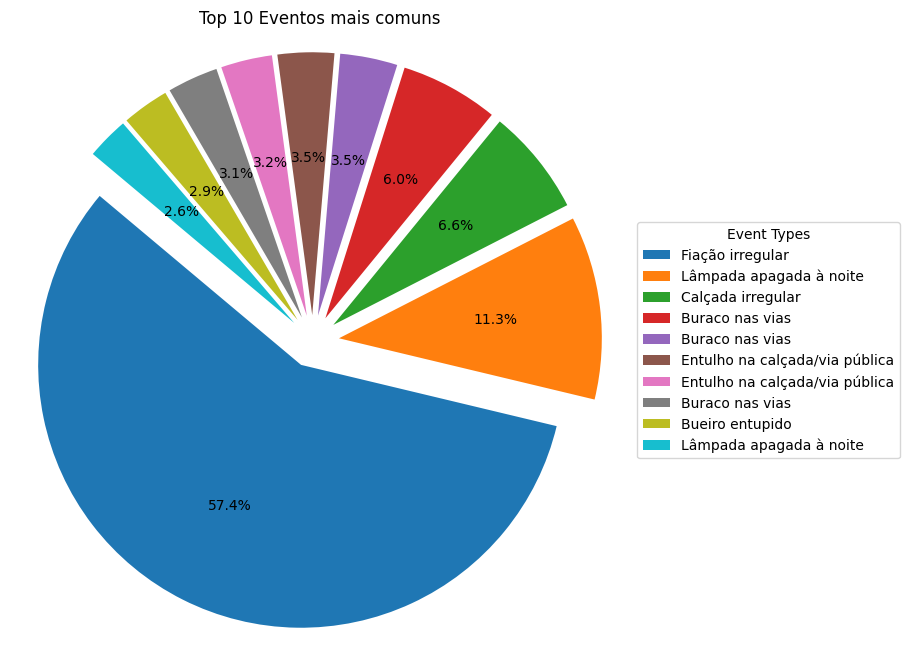
\includegraphics[width=0.8\textwidth]{images/pie_most_common_events.png}
	\fautor
\end{quadro}

Ao expandir nossa análise para considerar a dimensão de gênero, observamos padrões distintos na distribuição de sentimentos entre diferentes grupos. Para as usuárias identificadas como femininas, notamos que a maioria das postagens (8.207) tem um sentimento negativo, seguido por 3.894 postagens positivas e 3.531 neutras. Isso sugere que, embora as mulheres estejam ativamente envolvidas na plataforma, elas tendem a expressar mais preocupações ou insatisfações em suas postagens do que sentimentos positivos ou neutros. Os usuários masculinos, por outro lado, apresentam um padrão diferente. Com 56.011 postagens neutras, 34.836 negativas e 22.513 positivas, vemos que a maioria das postagens masculinas é neutra. Isso pode indicar que os homens na plataforma tendem a ser mais informativos ou questionadores em suas postagens, sem expressar uma opinião clara em uma direção ou outra. Quanto aos usuários não binários, a amostra é extremamente pequena, com apenas uma postagem neutra registrada. Isso pode ser devido a uma representação limitada desse grupo na plataforma ou à relutância em se identificar devido a preocupações de privacidade. Os usuários que optaram por não informar seu gênero ou se identificaram como "outros" também têm uma presença na plataforma, embora em números menores em comparação com os gêneros masculino e feminino. Para os não informados, a distribuição é de 101 postagens negativas, 42 positivas e 37 neutras. Já para os que se identificam como "outros", temos 1.780 postagens negativas, 526 positivas e 1.356 neutras.

Essa análise por gênero destaca a importância de considerar as diversas perspectivas e experiências dos usuários ao avaliar o sentimento nas postagens. Cada grupo traz uma lente única para a plataforma, e entender essas nuances pode ajudar a criar estratégias de engajamento mais eficazes e a responder de forma mais adequada às preocupações e feedbacks dos usuários.

\begin{quadro}[!htb]
	\caption{Distribuição dos scores de sentimento por gênero.}
	\label{fig:sentiment_by_gender}
	\centering
	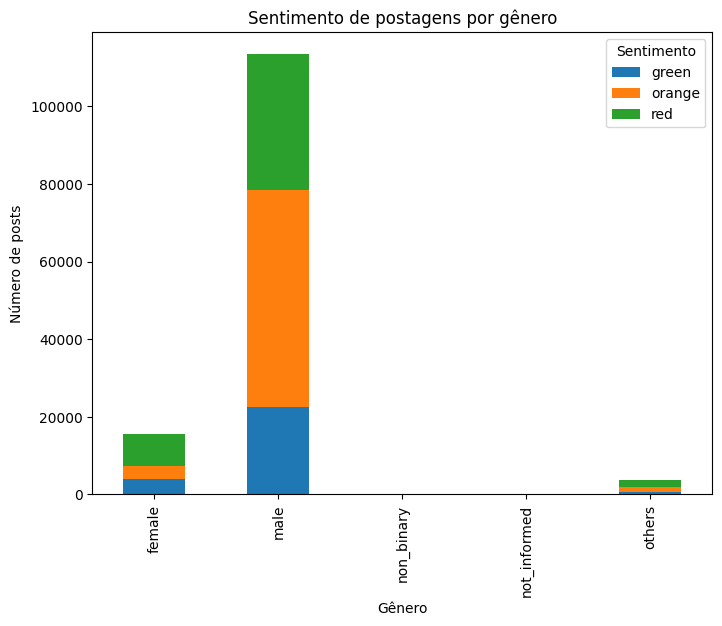
\includegraphics[scale=0.8]{images/sentiment_by_gender.png}
	\fautor
\end{quadro}

Aprofundando ainda mais nossa análise, decidimos explorar a relação entre a análise de sentimentos e a estrutura da rede social do Colab. A ideia era entender como os sentimentos expressos nas postagens poderiam influenciar ou ser influenciados pelas conexões e interações entre os usuários. Neste contexto, a análise de redes sociais, combinada com a análise de sentimentos, pode oferecer insights valiosos sobre a formação e a dinâmica de câmaras de eco dentro da plataforma.

Um conceito fundamental na análise de redes é a assortatividade, que mede a tendência de nós em uma rede se conectarem a outros nós que são semelhantes em alguma característica específica. No nosso caso, estávamos interessados em entender se usuários com sentimentos semelhantes tendem a se conectar e interagir mais entre si.

\begin{table}[h]
	\centering
	\begin{tabular}{|l|c|}
		\hline
		\textbf{Atributo} & \textbf{Valor de Assortatividade} \\
		\hline
		Tipo de Evento    & 0.015                             \\
		\hline
		Idade             & 0.015                             \\
		\hline
		Gênero            & 0.025                             \\
		\hline
		Escolaridade      & 0.01987                           \\
		\hline
		Raça              & 0.025                             \\
		\hline
		Score Lexicon     & 0.01489                           \\
		\hline
		Score Composto    & 0.01489                           \\
		\hline
		Score Positivo    & 0.01487                           \\
		\hline
		Score Negativo    & 0.01489                           \\
		\hline
		Score Neutro      & 0.01489                           \\
		\hline
		Cidade            & 0.02506                           \\
		\hline
	\end{tabular}
	\caption{Assortatividade por Atributo}
\end{table}

Para entender a influência dos sentimentos nas conexões entre os usuários, começamos por calcular a assortatividade da rede em relação a várias características, incluindo o tipo de evento, idade, gênero, educação, raça, score médio de sentimento e cidade. A assortatividade nos fornece uma métrica quantitativa que indica se a rede exibe uma tendência de homofilia, ou seja, se nós semelhantes tendem a se conectar entre si.

Os resultados foram reveladores. Os resultados foram reveladores. A assortatividade para todas as características listadas variou entre 0.01487 e 0.02506, indicando uma tendência moderada de homofilia na rede. Em outras palavras, há uma leve tendência para usuários com características semelhantes se conectarem entre si.

O atributo 'gênero' e 'raça' apresentaram valores de assortatividade de 0.025, sugerindo que os usuários tendem a se conectar mais frequentemente com outros usuários do mesmo gênero ou raça. Da mesma forma, o atributo 'cidade' também apresentou um valor semelhante de 0.02506, indicando que os usuários têm uma propensão a se conectar com outros que residem na mesma cidade. Isso era esperado, pois é natural que usuários da mesma cidade tenham mais probabilidade de se conectar e interagir entre si, dada a proximidade geográfica e os problemas comuns enfrentados.

Estes resultados têm implicações significativas para a dinâmica da rede social do Colab. A formação de câmaras de eco, especialmente em relação ao sentimento expresso nas postagens, pode influenciar a disseminação de informações, a percepção dos problemas e as soluções propostas. Por exemplo, se um grupo de usuários consistentemente posta com um sentimento negativo sobre um determinado tipo de evento, isso pode influenciar a percepção de outros usuários sobre a gravidade ou prevalência desse problema. Além disso, a presença de câmaras de eco pode ter implicações para a eficácia das intervenções ou políticas implementadas com base no feedback dos usuários. Se a plataforma estiver dominada por vozes particularmente positivas ou negativas, isso pode distorcer a percepção dos tomadores de decisão sobre as necessidades e prioridades da comunidade.

\begin{quadro}[!htb]
	\caption{Assortatividade por Atributo}
	\label{fig:assortativity_by_attribute}
	\centering
	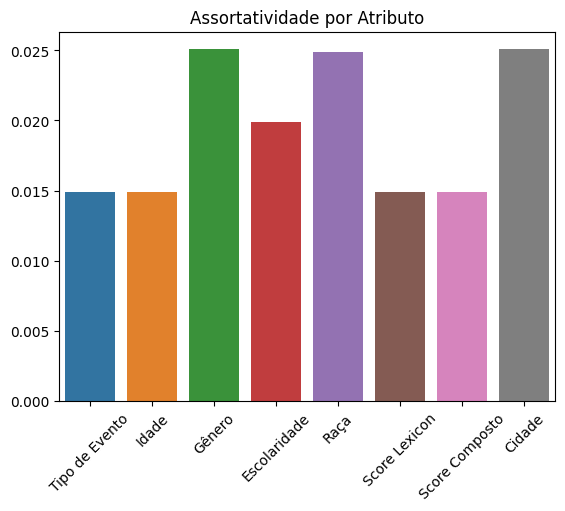
\includegraphics[scale=0.75]{images/assortativity_by_attribute.png}
	\fautor
\end{quadro}

Ao analisar os dez usuários com o maior número de postagens na rede, podemos identificar padrões e características que nos ajudam a entender melhor a dinâmica da plataforma e os comportamentos dos usuários mais ativos. Estes usuários, devido à sua alta atividade, têm o potencial de influenciar significativamente a percepção e o sentimento geral da comunidade.

\begin{table}[h]
	\centering
	\caption{Detalhes dos usuários mais ativos}
	\begin{tabular}{|c|c|c|c|c|c|c|c|c|}
		\hline
		ID     & Centralidade & Seguidores & Seguindo & Eventos & Score & Gênero & Idade & Raça \\
		\hline
		318649 & 0.0585          & 24         & 5        & 12287.0   & -0.011      & M      & 38    & -    \\
		\hline
		240336 & 0.0532          & 13         & 4        & 11609.0   & 0.03        & M      & 49    & P    \\
		\hline
		425243 & 0.0422          & 15         & 15       & 5310.0    & -0.001      & M      & 48    & P    \\
		\hline
		216238 & 0.1354          & 72         & 17       & 4490.0    & -0.055      & M      & 59    & P    \\
		\hline
		186310 & 0.2552          & 133        & 406      & 4185.0    & -0.052      & M      & 52    & N    \\
		\hline
		76184  & 0.0447          & 74         & 56       & 4031.0    & -0.079      & M      & 31    & N    \\
		\hline
		43341  & 0.0261          & 64         & 24       & 3621.0    & -0.165      & M      & 40    & B    \\
		\hline
		194422 & 0.0234          & 28         & 14       & 2911.0    & -0.329      & O      & 28    & -    \\
		\hline
		253059 & 0.0624          & 26         & 6        & 1698.0    & 0.082       & M      & 48    & B    \\
		\hline
		200628 & 0.0341          & 43         & 0        & 1550.0    & -0.393      & M      & 36    & B    \\
		\hline
	\end{tabular}
\end{table}

Os dois usuários que lideram em número de postagens, com IDs 318649 e 240336, demonstram uma presença significativa na rede, com 12287 e 11609 postagens, respectivamente. No entanto, a influência na rede não se restringe apenas ao volume de postagens. A centralidade de autovetor, que indica a influência de um nó na rede, mostra que o usuário com ID 186310, apesar de estar em quinto lugar em número de postagens, é um dos mais influentes, com uma centralidade de 0.2552. Este usuário destaca-se não só pela sua influência, mas também pelo seu alto número de seguidores, 133, e pelo fato de seguir 406 outros usuários.

O sentimento geral das postagens, representado pelo score médio, varia entre os usuários. Por exemplo, enquanto o usuário com ID 253059 tem um score médio positivo de 0.082, indicando uma tendência a postagens mais positivas, o usuário com ID 194422 tem o score mais negativo de -0.329, sugerindo postagens com um tom mais crítico ou descontente.

Além disso, é interessante observar a diversidade demográfica entre os usuários mais ativos. Temos representantes de diferentes faixas etárias, desde os 28 anos do usuário com ID 194422 até os 59 anos do usuário com ID 216238. Em termos de raça, há uma variedade, com usuários identificados como brancos, negros e pardos. O gênero predominante entre os mais ativos é masculino, com uma exceção identificada como "outros".

A presença de uma ampla gama de scores de sentimento entre os usuários mais ativos é uma indicação saudável de uma comunidade vibrante e multifacetada. Em muitas plataformas online, é comum encontrar usuários que repetidamente postam conteúdo com uma única tonalidade, seja ela positiva, negativa ou neutra. No entanto, a diversidade observada aqui sugere que esses usuários estão engajados em uma variedade de tópicos e situações, refletindo uma gama mais ampla de experiências e sentimentos.

Além disso, essa variedade pode ser vista como um indicativo de autenticidade. Usuários que consistentemente postam com um único tom podem ser percebidos como tendenciosos ou até mesmo como bots. Por outro lado, aqueles cujas postagens refletem uma variedade de sentimentos são mais propensos a serem vistos como genuínos e confiáveis por outros membros da comunidade.

Isso também destaca a importância de não fazer suposições apressadas sobre os usuários com base apenas em sua atividade. Enquanto um alto volume de postagens pode sugerir um usuário muito engajado, a verdadeira natureza de seu engajamento só pode ser compreendida ao se considerar o conteúdo e o sentimento dessas postagens.

A diversidade de sentimentos também pode ser um indicativo de que a plataforma está servindo a seu propósito de fornecer um espaço para discussão e feedback. Se todos os usuários mais ativos tivessem sentimentos uniformemente positivos ou negativos, poderia ser um sinal de que a plataforma está se tornando uma câmara de eco, onde apenas certas opiniões são expressas e reforçadas.

Além disso, essa diversidade pode ser benéfica para os administradores ou moderadores da plataforma. Ao monitorar os sentimentos variados dos usuários mais ativos, eles podem obter insights valiosos sobre áreas de preocupação, bem como aspectos da plataforma ou da comunidade que estão funcionando bem. Isso pode informar decisões sobre modificações na plataforma, campanhas de engajamento ou iniciativas de moderação.

Por fim, é essencial reconhecer que, em qualquer comunidade, a diversidade de opiniões e experiências enriquece o diálogo e a troca de ideias. A presença de usuários ativos com uma variedade de sentimentos sugere uma comunidade dinâmica e engajada, onde os membros se sentem livres para expressar suas opiniões e compartilhar suas experiências, sejam elas positivas, negativas ou neutras.

\begin{quadro}[!htb]
	\caption{Eigencentrality vs. Número de Posts}
	\label{fig:eigencentrality_vs_number_of_posts}
	\centering
	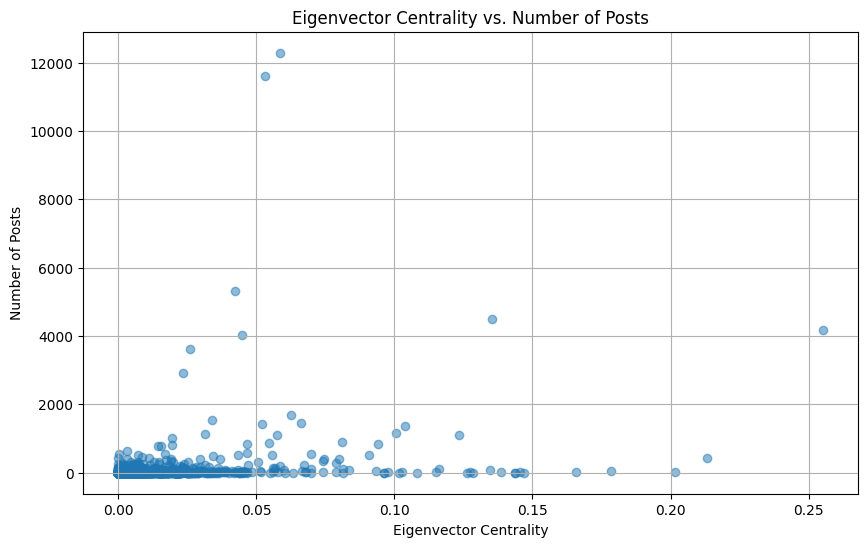
\includegraphics[scale=0.70]{images/eigencentrality_vs_number_of_posts.png}
	\fautor
\end{quadro}

Ao longo deste experimento, exploramos a o complexo microcosmo representado pelos sentimentos e opiniões expressas pelos usuários da plataforma Colab. A análise de sentimentos, quando aplicada a plataformas de mídia social, pode revelar insights profundos sobre as percepções, preocupações e satisfações dos usuários. No caso do Colab, essa análise nos permitiu entender melhor a dinâmica da comunidade e as emoções subjacentes às postagens dos usuários.

Primeiramente, a presença de uma distribuição quase equilibrada de sentimentos positivos e negativos desafia a noção comum de que plataformas de feedback tendem a ser dominadas por críticas. Isso sugere que o Colab não é apenas um espaço para reclamações, mas também um fórum onde os usuários reconhecem e apreciam as soluções e melhorias.

A análise dos usuários mais ativos e suas postagens revelou uma diversidade saudável de sentimentos, refutando a ideia de que os usuários mais ativos são unidimensionais em suas postagens. Esta diversidade é um testemunho da autenticidade e do engajamento genuíno dos usuários com a plataforma. Além disso, destaca a importância de considerar o conteúdo e o sentimento das postagens, em vez de se basear apenas no volume de atividade.

A presença de câmaras de eco, onde usuários com sentimentos semelhantes tendem a se agrupar, é uma preocupação em muitas plataformas online. No entanto, a diversidade de sentimentos observada no Colab sugere que a plataforma tem evitado, até certo ponto, essa armadilha. Isso é crucial para garantir que a plataforma continue a ser um espaço para discussão aberta e feedback construtivo.

A análise de redes sociais combinada com a análise de sentimentos também revelou padrões interessantes de conexão e interação entre os usuários. A tendência de usuários com sentimentos semelhantes se conectarem entre si tem implicações significativas para a disseminação de informações e a formação de opiniões dentro da plataforma.

Em conclusão, a análise de sentimentos no Colab ofereceu uma janela única para o coração e a mente da comunidade. Revelou uma comunidade vibrante e engajada, onde os membros se sentem empoderados para expressar suas opiniões e compartilhar suas experiências. À medida que a plataforma continua a crescer e evoluir, será essencial continuar monitorando e compreendendo esses sentimentos para garantir que o Colab permaneça um espaço inclusivo, autêntico e valioso para todos os seus membros.

\section{Análise de Sentimento com Regressão Supervisionada}
\label{sec:analise_de_sentimento_com_regressao_supervisionada}

Até o momento, nossa abordagem para a análise de sentimentos nas postagens do Colab foi baseada em técnicas manuais e ferramentas como o NLTK. Embora tenhamos obtido insights valiosos e estabelecido um score para cada postagem, é evidente que essa metodologia possui limitações em termos de escalabilidade e sustentabilidade, especialmente considerando o volume crescente de dados gerados diariamente na plataforma. Para superar esses desafios e otimizar o processo de análise de sentimentos, é imperativo adotar uma abordagem mais automatizada e robusta. Neste contexto, o aprendizado de máquina emerge como uma solução promissora. Ao utilizar um subconjunto das postagens que já classificamos manualmente - um conjunto de treinamento de aproximadamente 4.000 postagens - podemos treinar um modelo de aprendizado de máquina para realizar a classificação de sentimentos de forma autônoma. Esta abordagem não apenas acelera o processo de análise, mas também garante uma maior consistência e precisão na classificação. No próximo segmento, exploraremos em detalhes a implementação e os benefícios desta metodologia baseada em aprendizado de máquina, delineando como ela pode melhorar nossa capacidade de entender e interpretar os sentimentos expressos pelos usuários do Colab.

Nessa seção, descrevemos a metodologia empregada para a análise de dados e a construção do modelo de aprendizado de máquina e apresentamos uma abordagem para realizar a análise de sentimento em postagens do Colab. Este modelo foi treinado usando um conjunto de dados de treinamento que consiste em postagens de usuário rotuladas como positivas ou negativas. O modelo então aprende a associar certas palavras e frases a sentimentos positivos ou negativos.

A distinção entre classificação e regressão é um pilar central no aprendizado de máquina supervisionado. A classificação é destinada à atribuição de categorias discretas a instâncias de dados, ao passo que a regressão prediz elementos contínuos, oferecendo um espectro de possibilidades (\citeonline{2017_Shen_IC}).

No domínio da análise de sentimentos, a prática convencional muitas vezes simplifica a complexidade dos sentimentos humanos a categorias binárias. Todavia, sentimentos são intrinsecamente graduais e multidimensionais. Ao adotar uma escala contínua de -1 a 1 para representar sentimentos, abraçamos a sutileza e a riqueza dessas variações.

A opção pela regressão como abordagem modelagem foi catalisada pelos insights revelados na análise exploratória de sentimentos do capítulo anterior, na qual identificamos um espectro completo de sentimentos. Preservar essa continuidade permite-nos capturar as nuances mais finas nas postagens, concedendo-nos também a flexibilidade para futuras adaptações metodológicas sem a perda de detalhes valiosos dos dados originais.

Para fortalecer nosso conjunto de dados de treinamento e expandir nossa compreensão dos sentimentos manifestados nas postagens do Colab, incluímos uma seleção aleatória de 2000 eventos adicionais. Esta estratégia promove a diversidade e representa melhor a gama de sentimentos expressos, evitando vieses que poderiam surgir da seleção de extremos. Combinando esses eventos com os dados das postagens das três cidades estudadas anteriormente, consolidamos um conjunto de treinamento robusto com 4000 instâncias.

Esperamos que o algoritmo, ao ser treinado com essa rica fonte de dados, aprenda a correlacionar padrões linguísticos com sentimentos positivos ou negativos, propiciando uma classificação automática refinada dos sentimentos nas postagens do Colab. Esta abordagem de aprendizado supervisionado utiliza os dados de treinamento como alicerces para a criação de um modelo generalista capaz de captar a gama de sentimentos expressos nas postagens.

Depois da extração de recursos e da análise exploratória, dividimos os dados em conjuntos de treino e validação, seguido pela padronização dos mesmos para assegurar uniformidade na escala (\cite{2000_Jain}). Testamos uma gama de modelos regressivos para discernir o mais apropriado para nossa aplicação:

\begin{itemize}
\item \textbf{RandomForestRegressor}: Este algoritmo constrói um ensemble de árvores de decisão e usa a média de suas previsões para gerar o resultado final. É notável pela sua robustez em lidar com grandes volumes de dados e pela habilidade em captar interações complexas entre as variáveis, minimizando o risco de overfitting \cite[5-32]{2001_Breiman}.
\item \textbf{LinearRegression}: Um dos métodos mais fundamentais e amplamente aplicados, a Regressão Linear busca estabelecer uma relação linear entre variáveis dependentes e independentes.
\item \textbf{DecisionTreeRegressor}: Este modelo segmenta o espaço de dados em subconjuntos baseados em características e utiliza a média dos valores dos subconjuntos para fazer previsões. Sua interpretabilidade é uma vantagem, embora possa sucumbir ao overfitting se não for devidamente ajustado \cite[81-106]{1986_Quinlan}.
\item \textbf{K-Nearest Neighbors (KNN)}: O KNN faz previsões com base na semelhança entre instâncias de dados, considerando os 'k' exemplos mais próximos no conjunto de treinamento para inferir resultados.
\end{itemize}

Em um campo desafiador como a análise de sentimentos, especialmente quando focado na identificação de câmaras de eco, é imperativo selecionar um modelo de aprendizado de máquina que possa capturar com precisão a gama de sentimentos nos dados. Avaliamos o desempenho dos modelos utilizando métricas como MSE, MAE e o coeficiente de determinação (R\^2), que são mais indicativas do que a acurácia para tarefas de regressão.

O Random Forest Regressor destaca-se como a opção mais promissora, exibindo um equilíbrio ideal entre acurácia e generalização. O Decision Tree Regressor, apesar de um R\^2 quase perfeito no treinamento, evidencia overfitting devido à discrepância em validação. O KNN não alcançou o desempenho esperado em comparação aos outros modelos.

\begin{table}[h]
	\centering
	\begin{tabular}{|l|c|c|c|c|c|c|}
		\hline
		\textbf{Modelo} & \textbf{Training R$^2$} & \textbf{Validation R$^2$} & \textbf{MSE} & \textbf{MAE} & \textbf{RMSE} & \textbf{Tempo (s)} \\
		\hline
		Random Forest   & 0.9619                  & 0.7228                    & 0.0847       & 0.1683       & 0.2910        & 1192.96            \\
		\hline
		Decision Tree   & 0.9999                  & 0.5107                    & 0.1496       & 0.1894       & 0.3867        & 33.65              \\
		\hline
		KNN             & 0.4932                  & 0.1727                    & 0.2529       & 0.3871       & 0.5029        & 133.97             \\
		\hline
	\end{tabular}
	\caption{Desempenho dos modelos de regressão nos dados de treinamento e validação.}
	\label{tab:model_performance}
\end{table}	

A partir desses resultados, podemos concluir que o Random Forest Regressor é o modelo mais promissor entre os testados, com o melhor equilíbrio entre desempenho nos dados de treinamento e validação. O Decision Tree Regressor parece estar overfitting, dado o R\^2 quase perfeito nos dados de treinamento e o desempenho significativamente pior nos dados de validação. O KNN, por outro lado, tem um desempenho geralmente mais fraco em comparação com os outros modelos.

Em análise de sentimentos, a precisão é um desiderato, especialmente ao explorar dinâmicas sociais em plataformas como o Colab. Iniciamos este capítulo com um experimento nas mensagens dos usuários de três cidades, utilizando uma heurística baseada em dicionários de sentimentos, polaridade de emojis e ferramentas como o LeIA. A transparência dessa metodologia inicial é uma vantagem, mas também pode introduzir vieses. O trânsito para um modelo de aprendizado de máquina, especificamente o Random Forest, tem como objetivo mitigar tais vieses e melhorar a objetividade.

A preparação e a qualidade dos dados são vitais para o sucesso do modelo de aprendizado. Ao utilizar os scores de sentimentos do experimento inicial como entradas para o modelo regressivo, estabelecemos um processo sequencial e integrado de análises. Este estudo sublinha a importância de métodos adaptáveis na análise de sentimentos, especialmente ao lidar com fenômenos sociais complexos. Com os insights adquiridos, o próximo passo é classificar os usuários em personas, utilizando o score de sentimentos, tópicos de interesse e modelos de classificação para desvelar as tendências de polarização e interação no Colab.

A análise de sentimentos, particularmente em plataformas dinâmicas como o Colab, é uma tarefa intrincada que exige uma abordagem meticulosa. No início deste capítulo, conduzimos um experimento para classificar as mensagens dos usuários de Niterói, Santo André e Mesquita. Utilizando uma heurística baseada em dicionários léxicos, polaridade de emojis e a ferramenta LeIA, atribuímos scores de sentimentos às postagens. Este processo é transparente, permitindo-nos codificar cada etapa da atribuição de scores como uma caixa branca. No entanto, essa transparência também pode introduzir viéses, sejam eles conscientes ou não.

A decisão de transformar essa abordagem inicial em um modelo de aprendizado de máquina foi motivada pela perspectiva da engenharia de software. Ao adotar a regressão supervisionada, buscamos criar um sistema mais objetivo e menos suscetível a viéses humanos. A escolha do Random Forest Regressor, que demonstrou desempenho superior, reitera a necessidade de algoritmos robustos para capturar padrões complexos nos dados. Além disso, manter os scores de sentimento em um espectro contínuo, em vez de categorias discretas, permitiu uma representação mais fiel e granular dos sentimentos.

A qualidade dos dados e sua preparação são fundamentais para o sucesso de qualquer modelo de aprendizado de máquina. Ao usar os scores de sentimentos derivados do experimento inicial como insumo para o treinamento do modelo de regressão, demonstramos a interconexão e a sequencialidade dos experimentos. Esta pesquisa destaca a importância de abordagens adaptativas em análise de sentimentos, especialmente ao abordar fenômenos sociais complexos. Com os insights obtidos através desta modelagem de sentimentos, o próximo passo é a classificação dos usuários em personas. Utilizando o score de sentimento, os tópicos mais comentados e um modelo de classificação, buscaremos entender melhor os perfis dos usuários. Esta compreensão será crucial para a subsequente análise de redes, visando a detecção de câmaras de eco e aprofundando nossa compreensão sobre as dinâmicas de interação e polarização no Colab.

\section{Análise de Sentimento e Personas: Uma Nova Perspectiva sobre as Postagens do Colab}

Nossa jornada analítica no Colab começou com uma avaliação meticulosa das interações dos usuários, empregando técnicas sofisticadas de processamento de linguagem natural e análise de redes. Este processo gerou um sistema de pontuação capaz de capturar a polaridade dos sentimentos - positivos, negativos ou neutros - em cada postagem. Esta avaliação considerou não só o léxico e emojis utilizados, mas também os jargões e nuances específicas da plataforma.

Este sistema não só desvendou a natureza das interações na plataforma, revelando tendências e sentimentos dominantes, como também permitiu, ao ser combinado com análise de redes, vislumbrar a disseminação de sentimentos através das conexões entre os usuários. Esta sinergia entre análise de sentimentos e de redes elucidou a dinâmica complexa das interações comunitárias.

Com a análise de sentimentos estabelecida, o foco ampliou-se naturalmente para a classificação de personas, com o intuito de decifrar padrões comportamentais mais abrangentes dos usuários. Esta etapa avançada da pesquisa almejou transcender a análise individual de postagens para compreender como os usuários, em suas conexões e influências mútuas, coalescem em arquétipos mais amplos - as personas.

Essas personas são construções representativas que sintetizam os traços e comportamentos de grupos de usuários. No ecossistema do Colab, identificamos principalmente duas personas: os \textit{helpers} e os \textit{complainers}. Os Helpers se caracterizam pelo engajamento colaborativo e proativo, frequentemente auxiliando e partilhando informações valiosas. Já os Complainers tendem a adotar uma postura mais crítica, expressando descontentamento e críticas frequentes.

Ambas as personas são fundamentais para a dinâmica do Colab. Os Helpers fomentam o apoio mútuo e a resolução colaborativa de problemas, enquanto os Complainers podem ser catalisadores de mudança, destacando áreas que necessitam de atenção e melhoria. Contudo, quando essas personas se polarizam, surgem riscos de formação de câmaras de eco, locais onde as opiniões se reforçam mutuamente, limitando a diversidade de perspectivas.

Através da análise de sentimentos e subsequente classificação em personas, procuramos desvendar como os usuários se distribuem na rede do Colab e os padrões emergentes. Esse entendimento é crucial para identificar a existência de "bolhas de personas" e para investigar a dinâmica que as sustenta: Será um fenômeno intrínseco ao comportamento dos usuários ou as plataformas de mídia social estão, através de viéses algorítmicos, contribuindo ativamente para essa segregação? No decorrer desta seção, abordaremos as metodologias aplicadas para discernir e classificar as personas \textit{helpers} e \textit{complainers} no Colab. Ao aprofundar-se na implementação desses arquétipos, realçaremos sua relevância para a análise de dados e para o aprimoramento estratégico da plataforma.

\subsection{Helpers}

A persona \textit{helper} é caracterizada por um comportamento proativo e colaborativo em uma comunidade online. Esses indivíduos são frequentemente encontrados respondendo a perguntas, oferecendo conselhos e compartilhando informações úteis com outros membros da comunidade. Eles tendem a expressar sentimentos positivos em suas postagens e são motivados pelo desejo melhorar o coletivo e contribuir para a comunidade.

No Colab, por exemplo, muitos usuários realizam postagens frequentes reportando buracos nas vias, estruturas danificadas, alertam para situações de alagamento e deslizamento de terrenos. Muitos desses usuários adotam formatos padronizados para suas postagens, incluindo fotos, localização e descrição detalhada do problema. Além disso, eles frequentemente interagem com outros usuários, fornecendo informações adicionais ou atualizações sobre o status do problema.

Os \textit{helpers} são fundamentais para o sucesso de qualquer comunidade online, pois eles ajudam a criar um ambiente de apoio e colaboração. Eles são frequentemente vistos como líderes informais ou especialistas em suas respectivas áreas de interesse. Eles podem ser motivados por uma variedade de fatores, incluindo o desejo de compartilhar conhecimento, a satisfação de ajudar os outros, ou o reconhecimento e respeito que recebem da comunidade.

\subsection{Complainers}

A persona \textit{complainer} é caracterizada por um comportamento mais crítico ou negativo em uma comunidade online. Esses indivíduos são frequentemente encontrados expressando insatisfação, fazendo reclamações ou criticando ações das agências públicas. Eles tendem a expressar sentimentos negativos em suas postagens e são motivados por uma variedade de fatores, incluindo frustração, descontentamento ou a necessidade de expressar suas opiniões. Também é importante notar que a maioria das postagens de \textit{complainers} não são necessariamente negativas, pois os usuários estão de fato reportando problemas nas cidades, mas podem ser percebidas como tal devido ao seu tom ou conteúdo. Um outro fator interessante é que muitas das postagens de \textit{complainers} são direcionadas a assuntos mais individualizados como reportes nas vicinidades de suas residências ou locais de trabalho. Notavelmente ao analisar os comentários, esses usuários tendem a comentar ativamente em postagens criadas por outros usuários, muitas vezes expressando apoio ou concordância com o autor da postagem, mas sempre destacando a ineficiência ou ineficácia dos órgãos públicos.

No Colab, muitos usuários realizam postagens se referindo a prefeitura e outros órgãos sarcasticamente, fazendo críticas e reclamações sobre a falta de manutenção de vias, atrasos em obras, entre outros. Outro ponto recorrente diz respeito a perturbação sonora e uma certa correlação com alguns preconceitos musicais. Alguns usuários com scores particularmente negativos tendem a cobrar os orgãos públicos pelos impostos pagos que são, na opinião desses usuários, mal administrados, assim como outras tarifas como de transporte público ou de energia elétrica.

Os \textit{complainers} desempenham um papel importante em qualquer comunidade online, pois eles ajudam a identificar problemas, desafios ou áreas de melhoria. Embora suas postagens possam ser percebidas como negativas, elas podem fornecer feedback valioso que pode ser usado para melhorar a comunidade. No entanto, é importante gerenciar e responder adequadamente a esses usuários para evitar a criação de um ambiente negativo ou tóxico.

\subsection{Personas e papéis nas comunidades do Colab}

A presença das personas \textit{helpers} e \textit{complainers} dentro do Colab é altamente relevante para o ecossistema dessa plataforma colaborativa. Ambas as personas desempenham papéis distintos e complementares que podem influenciar a experiência do usuário e fornecer insights valiosos para o aprimoramento contínuo do aplicativo. A seguir, são apresentados os argumentos que sustentam a relevância dessas personas específicas:

Os Helpers desempenham um papel fundamental no Colab, pois contribuem ativamente para a comunidade, oferecendo suporte, compartilhando conhecimento e fornecendo soluções para os desafios enfrentados pelos usuários. Eles ajudam a fomentar a colaboração e o aprendizado coletivo, tornando-se recursos valiosos para aqueles que precisam de assistência ou orientação. Sua presença cria um ambiente propício para troca de ideias, resolução de problemas e crescimento mútuo. Ao compartilhar suas habilidades e conhecimentos, os Helpers estabelecem uma cultura de generosidade e reciprocidade dentro da comunidade do Colab. Eles inspiram outros usuários a se envolverem ativamente, encorajando a participação e a colaboração entre os membros. Além disso, a presença de Helpers é essencial para garantir que novos usuários se sintam bem-vindos e apoiados, promovendo assim um ambiente inclusivo e acolhedor.

Embora os Complainers possam ser vistos como usuários críticos ou negativos, sua presença é igualmente importante para o Colab. Essas personas desempenham o papel de destacar problemas, lacunas e áreas de melhoria dentro do aplicativo. Ao expressar suas preocupações e insatisfações, eles fornecem um feedback valioso que pode impulsionar o aprimoramento contínuo da plataforma.

Os Complainers atuam como "sentinelas" da comunidade, chamando a atenção para questões que podem ter sido negligenciadas ou passado despercebidas. Suas críticas construtivas podem levar a melhorias significativas na usabilidade, funcionalidade e qualidade geral do Colab. Além disso, ao abordar e resolver essas preocupações, a equipe responsável pelo desenvolvimento do aplicativo demonstra seu compromisso com a satisfação e o engajamento dos usuários.

A interação entre as personas \textit{helpers} e \textit{complainers} no Colab é uma relação simbiótica que impulsiona o crescimento e o aprimoramento contínuo da plataforma. Os Helpers oferecem suporte, orientação e soluções, tornando o ambiente colaborativo e enriquecedor. Por outro lado, os Complainers fornecem feedback crítico e identificam áreas de melhoria, promovendo a evolução e aprimoramento do aplicativo. Essa sinergia entre essas personas complementares é essencial para criar uma comunidade vibrante, responsiva e em constante aprimoramento no Colab.

A partir de uma análise exploratória de sentimento, foram identificadas as personas \textit{helpers} e \textit{complainers} dentro do Colab. No entanto, é importante ressaltar que existem outras personas que também podem ser identificadas, como por exemplo, a persona "Explorer", que tem um perfil voltado para a exploração da cidade e reporte dos problemas identificados. Além disso, uma nova persona que poderia ser considerada é a persona "Innovator", alguém que está sempre em busca de novas soluções e ideias inovadoras para melhorar a experiência dos usuários no Colab. A escolha das duas personas mencionadas anteriormente foi baseada nossa capacidade de mensurar e classificar essas personas através da analise de sentimento de suas postagens e também em seu potencial de gerar câmaras de eco, pois representam posições mais antagônicas dentro das comunidades da rede.

Nas próximas páginas, detalharemos as técnicas e metodologias utilizadas para identificar e classificar as personas \textit{helpers} e \textit{complainers} dentro do Colab, fornecendo uma visão mais aprofundada sobre a implementação dessas personas e sua contribuição para a análise de dados e aprimoramento da plataforma.

\section{Classificação de usuário por Persona}

A construção de um modelo de classificação para análise de sentimentos em plataformas como o Colab é uma tarefa intrincada. A linguagem utilizada pelos usuários é repleta de nuances, jargões específicos, emojis e outros elementos que podem influenciar a interpretação do sentimento. Além disso, a diversidade demográfica dos usuários traz uma riqueza de perspectivas e formas de expressão. O principal desafio é desenvolver um modelo que seja sensível a essas nuances, evitando o overfitting, e que possa generalizar bem para postagens não vistas anteriormente.

Para assegurar uma representação abrangente e equitativa da comunidade do Colab, 5000 postagens foram meticulosamente selecionadas com base em critérios demográficos. Esta seleção garantiu que todas as faixas etárias, gêneros e raças estivessem representados de forma proporcional à distribuição desses grupos entre os usuários do aplicativo. Além disso, levamos em consideração o tamanho das postagens, garantindo uma mistura de postagens longas e curtas. Cada postagem foi então manualmente classificada como \textit{helper} ou \textit{complainer}, considerando-se o conteúdo, a intenção e as nuances da linguagem.

Do conjunto inicial de postagens, 4000 foram destinadas ao treinamento, mantendo um equilíbrio de 2000 postagens para cada categoria (\textit{helper} e \textit{complainer}). As 1000 postagens restantes foram reservadas como conjunto de teste. Esta separação assegura que o modelo seja treinado e avaliado em conjuntos distintos, minimizando o risco de overfitting.

\section{Análise de Redes baseada em Persona}

A jornada até aqui foi marcada por uma série de experimentos meticulosos, todos com um objetivo comum: construir heurísticas robustas para a detecção de câmaras de eco na rede do Colab. Através da aplicação do modelo de classificação, conseguimos uma visão detalhada das personas dos usuários, revelando nuances sobre como eles interagem e se expressam na plataforma. Esta análise nos mostrou que, apesar de existirem críticos e insatisfeitos, a maioria dos usuários busca colaborar e contribuir de forma positiva.

Ao integrar essas personas na análise de redes, conseguimos ir além da simples classificação. Observamos como as personas se manifestam na estrutura da rede, como se conectam e quais posições ocupam. Esta análise nos deu insights valiosos sobre a dinâmica das interações e sobre como diferentes tipos de usuários influenciam e são influenciados dentro da rede.

No entanto, o mais importante é o que fazemos com esses insights. A detecção de câmaras de eco é mais do que um exercício acadêmico; é uma busca para entender como as opiniões são formadas e reforçadas em ambientes digitais. Ao identificar e compreender essas câmaras, temos a oportunidade de promover diálogos mais abertos e inclusivos, onde diferentes vozes são ouvidas e onde a informação circula de forma mais equilibrada. Com os resultados obtidos, estamos um passo mais perto de tornar o Colab, e outras plataformas digitais, espaços mais saudáveis e representativos para todos os seus usuários.

\section{Aplicação e resultados do Modelo de Classificação}

Após a meticulosa construção e validação do modelo de classificação, chegou o momento de aplicá-lo ao conjunto de dados real e observar sua capacidade em campo. Utilizamos a rede composta pelas três cidades com maior interação, conforme identificado no \autoref{chapter:06_exploratory}, e o dataset contendo postagens dos usuários dessas cidades relacionadas a eventos de zeladoria pública. Ao rodar o modelo em todas as postagens, cada uma recebeu um score de sentimento e uma persona atribuída. Posteriormente, para determinar a persona de cada usuário, compilamos todas as postagens classificadas desse usuário e, através de uma média, calculamos sua persona predominante. Esta abordagem nos permite não apenas entender o sentimento expresso em postagens individuais, mas também obter uma visão mais ampla do perfil comportamental dos usuários no Colab.

\begin{quadro}[htb]
    \centering
    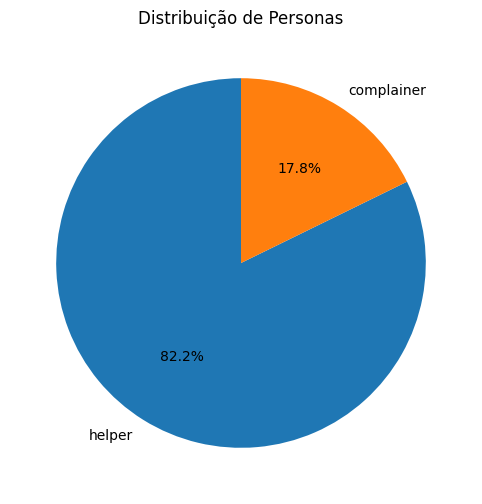
\includegraphics[width=0.5\textwidth]{images/personas_pie.png}
    \caption{Distribuição de Personas}
    \label{fig:personas_pie}
\end{quadro}

\begin{quadro}[htb]
    \centering
    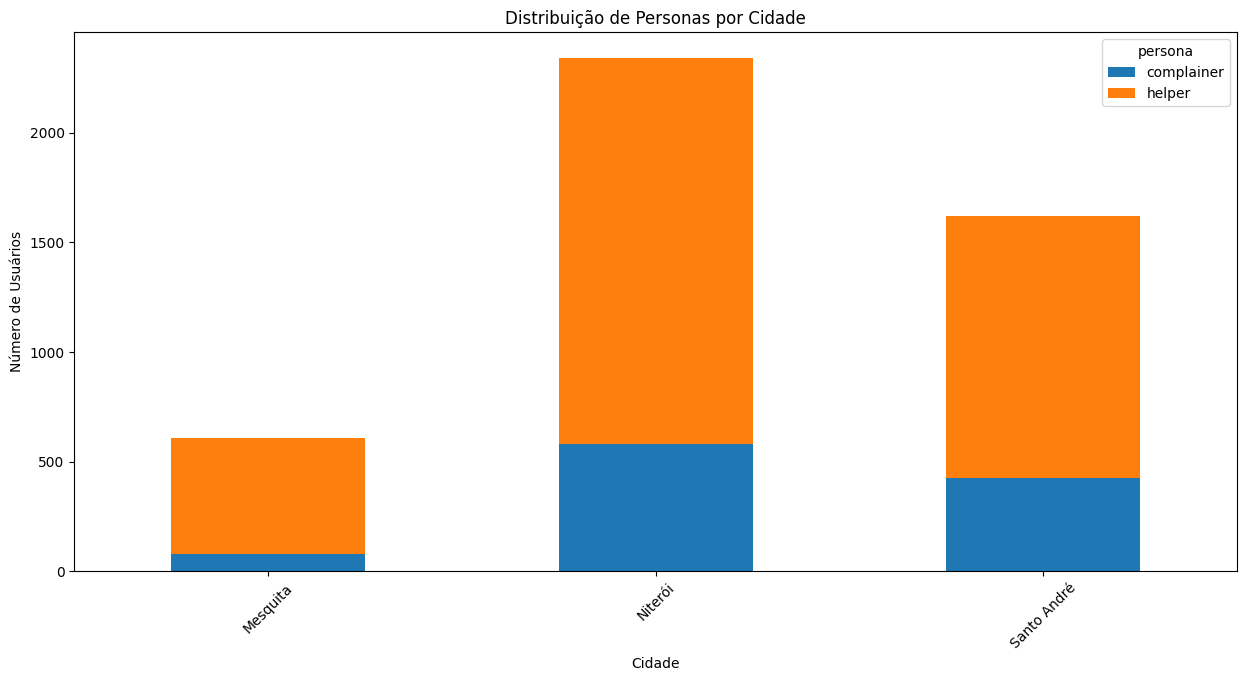
\includegraphics[width=0.95\textwidth]{images/personas_city.png}
    \caption{Distribuição de Personas por Cidade}
    \label{fig:personas_city}
\end{quadro}

A distribuição de personas revela uma predominância de usuários classificados como \textit{helper} (82.2\%) em comparação aos \textit{complainer} (17.8\%). Esta distribuição sugere que a maioria dos usuários do Colab tende a ser mais colaborativa e propositiva em suas postagens, enquanto uma minoria expressa insatisfações ou críticas. 

\begin{quadro}[htb]
    \centering
    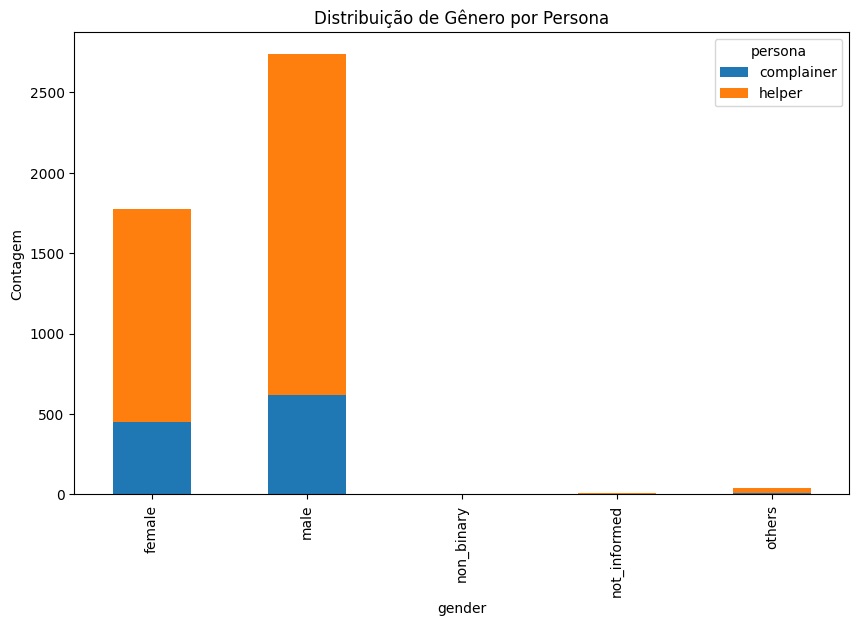
\includegraphics[width=0.7\textwidth]{images/persona_gender.png}
    \caption{Distribuição de Personas por Gênero}
    \label{fig:persona_gender}
\end{quadro}

\begin{quadro}[htb]
    \centering
    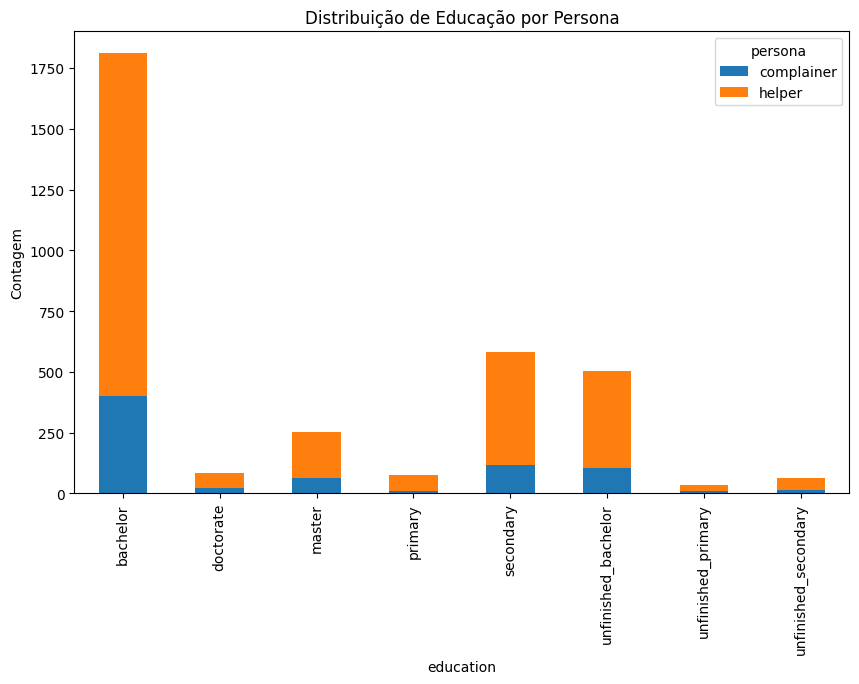
\includegraphics[width=0.7\textwidth]{images/persona_education.png}
    \caption{Distribuição de Personas por Escolaridade}
    \label{fig:persona_education}
\end{quadro}

\begin{quadro}[htb]
    \centering
    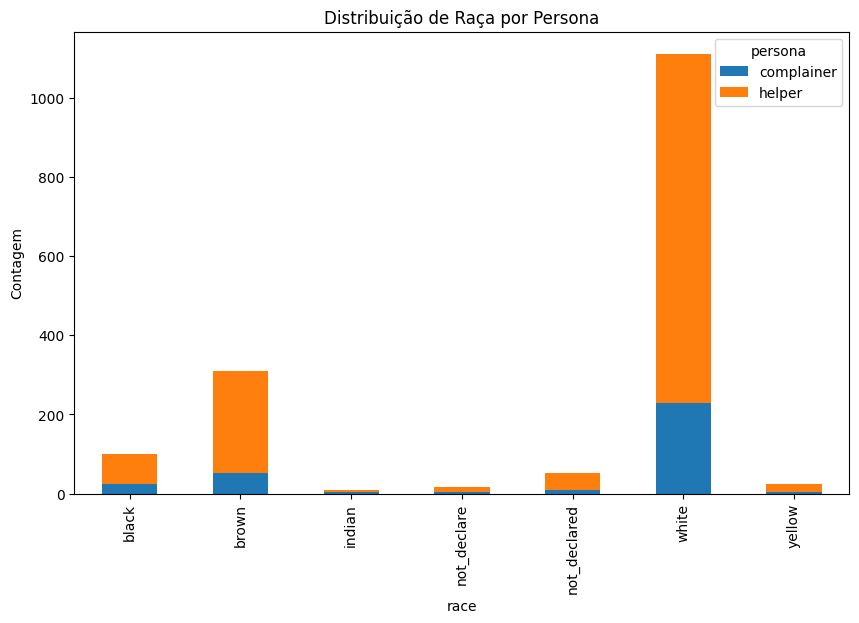
\includegraphics[width=0.7\textwidth]{images/persona_race.png}
    \caption{Distribuição de Personas por Raça}
    \label{f
	ig:persona_race}
\end{quadro}

Ao analisar a distribuição por cidade, observa-se que Niterói possui a maior proporção de \textit{helpers} (1759) em comparação com \textit{complainers} (582). Em contraste, Mesquita apresenta uma proporção mais equilibrada, com 532 \textit{helpers} e 78 \textit{complainers}. Santo André, por sua vez, segue uma tendência semelhante a Niterói, com 1194 \textit{helpers} e 424 \textit{complainers}. 

O espectro de gênero mostra que ambos os gêneros, masculino e feminino, têm uma proporção maior de \textit{helpers} em relação aos \textit{complainers}. No entanto, é interessante notar que, embora haja uma representação mínima de gêneros não binários e outros, eles também seguem essa tendência. 

Quando observamos a escolaridade, os usuários com formação de bacharelado lideram tanto na categoria \textit{helper} quanto na \textit{complainer}. No entanto, é notável que, em todas as categorias de escolaridade, os \textit{helpers} superam os \textit{complainers}. Em relação à raça, a maioria dos \textit{helpers} e \textit{complainers} se identifica como brancos, seguidos por pardos. As demais categorias raciais apresentam números menores, mas ainda assim, a tendência de mais \textit{helpers} do que \textit{complainers} persiste.

\begin{figure}[h]
    \centering
    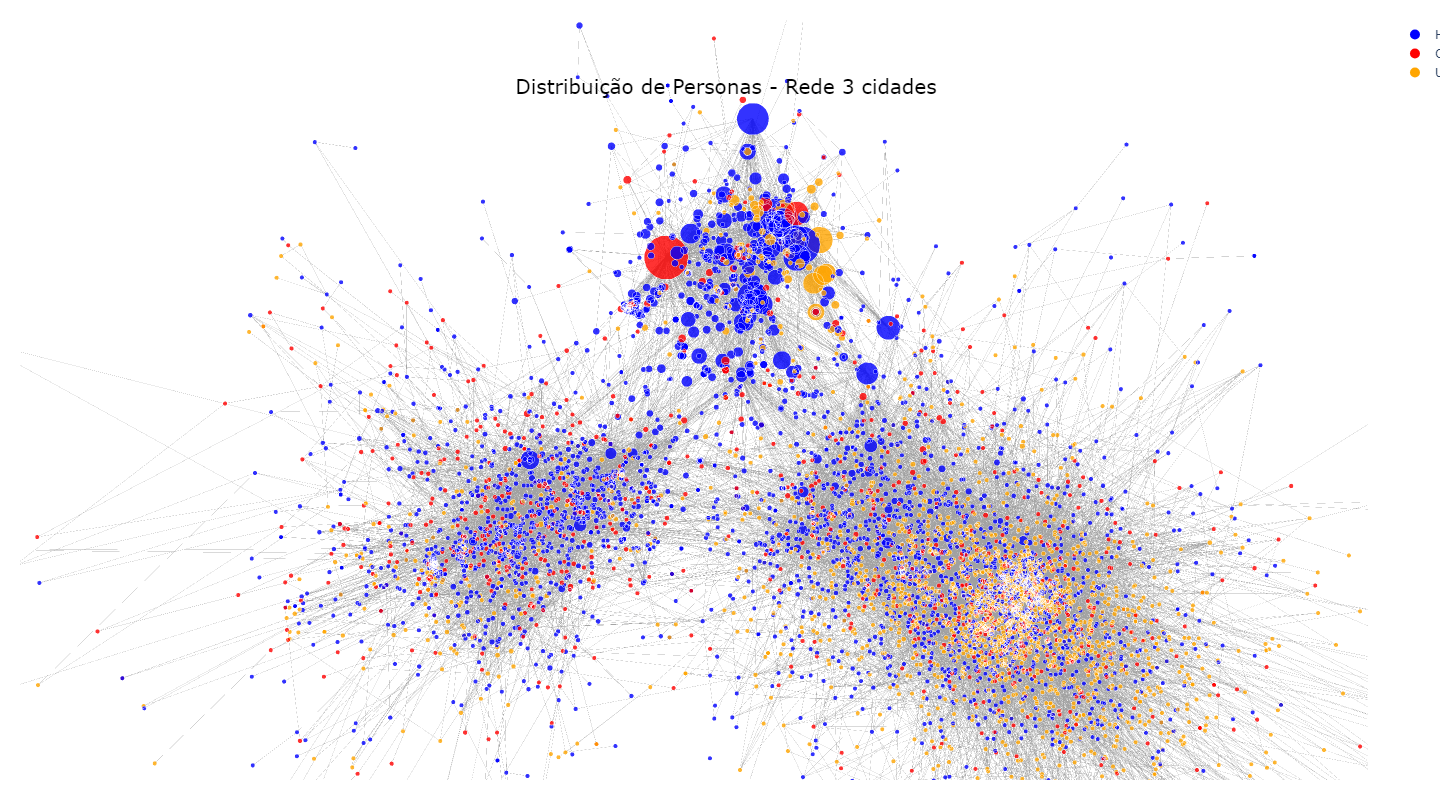
\includegraphics[width=1\textwidth]{images/personas_network.png} 
    \caption{Rede de usuários das 3 cidades com mais interações no Colab. Os usuários são agrupados de acordo com suas comunidades. Os nós são coloridos de acordo com a persona identificada: azul para helper, vermelho para complainer e laranja para não identificado.}
    \label{fig:personas_network}
\end{figure}

Após a classificação das postagens e a determinação das personas dos usuários, buscamos entender como essas personas se relacionam com a estrutura da rede de interações no Colab. A ideia é investigar se há padrões de comportamento ou tendências associadas a determinadas personas no contexto das interações na plataforma. Para isso, integramos o atributo de persona ao grafo, permitindo que cada nó (usuário) carregasse consigo sua persona predominante. Esta integração nos possibilita explorar correlações entre as métricas da rede e as personas, fornecendo insights sobre como diferentes tipos de usuários interagem e se posicionam dentro da rede.

A análise de redes revela um grafo direcionado com 6904 nós e 25785 arestas. A presença de 110 comunidades sugere uma estrutura de rede diversificada. A modulação, com uma pontuação de 0.6331, indica uma estrutura de comunidade bem definida. A assortatividade em relação à 'persona' é positiva (0.311), indicando que usuários com personas semelhantes tendem a se conectar entre si. Ao agrupar os nós da rede por 'persona', observa-se que, em média, os \textit{helpers} têm graus de entrada e saída mais altos e uma maior centralidade de eigenvector em comparação com os \textit{complainers}. Isso sugere que os \textit{helpers} podem ser mais centrais e influentes na rede do que os \textit{complainers}.

Ao combinar as métricas de análise de redes com as personas do usuário em uma matriz de correlação, percebemos que há uma relação positiva moderada entre o grau de entrada e o grau de saída. Na prática, o grau de entrada representa quantos usuários estão seguindo um determinado usuário, enquanto o grau de saída indica quantos usuários esse indivíduo está seguindo. Além disso, observa-se uma relação positiva entre o grau de entrada e a centralidade de eigenvector. A centralidade de eigenvector é uma métrica que identifica a influência de um nó na rede, considerando a qualidade das suas conexões. Ou seja, não apenas quantas conexões ele tem, mas também quão influentes são os nós com os quais ele está conectado.

Ao aprofundar a análise das métricas apresentadas, percebemos nuances distintas na distribuição e comportamento das personas nas três cidades em foco: Niterói, Santo André e Mesquita. A primeira observação notável é a variação na proporção de usuários classificados em cada cidade, sendo Mesquita e Santo André as que apresentam as maiores proporções, com aproximadamente 85\% de seus usuários classificados, enquanto Niterói possui cerca de 48\%.

\begin{figure}[h]
    \centering
    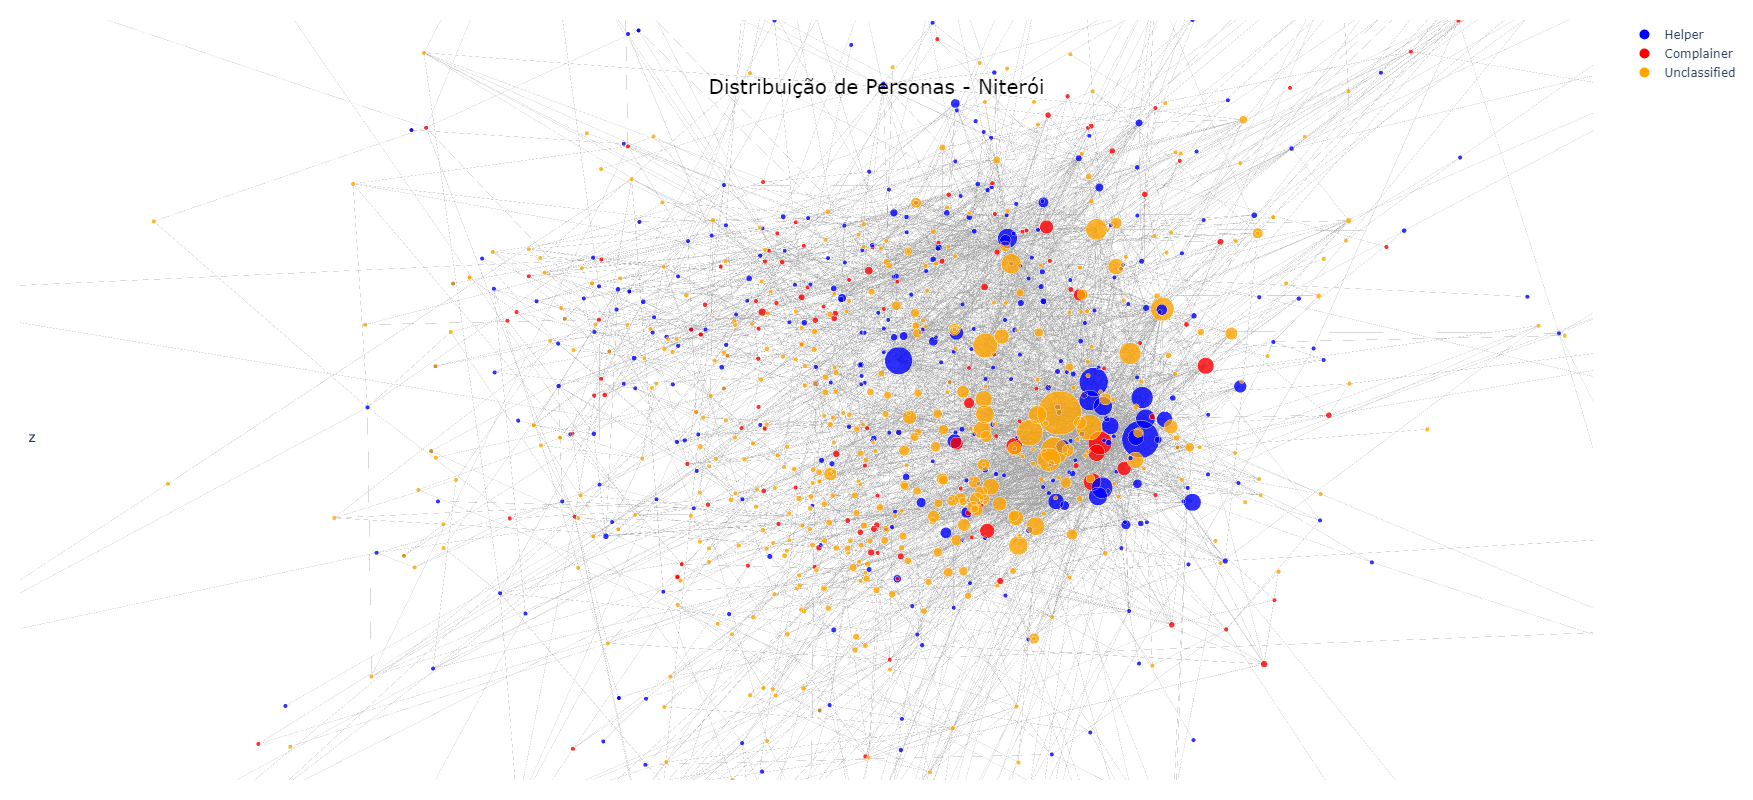
\includegraphics[width=1\textwidth]{images/network_personas_niteroi.png}
    \caption{Distribuição de personas na rede de usuários de Niterói.}
    \label{fig:network_personas_niteroi}
\end{figure}

Niterói, apesar de ter uma menor proporção de usuários classificados, mostra uma predominância significativa de \textit{helpers} sobre \textit{complainers}, uma característica compartilhada com Santo André. Mesquita, por outro lado, apresenta uma proporção ainda mais inclinada para \textit{helpers}, com 87,21\% de seus usuários classificados enquadrando-se nesta categoria. Este dado sugere que a dinâmica de interação em Mesquita pode ser mais colaborativa e positiva, o que pode influenciar a formação de comunidades e a disseminação de informações.

A análise da assortatividade em relação à 'persona' em cada cidade revela que usuários com personas semelhantes tendem a se conectar entre si, com a assortatividade variando de 0.007 em Niterói a 0.071 em Santo André. Este fenômeno pode ser um indicativo da formação de câmaras de eco, onde usuários com opiniões e comportamentos semelhantes tendem a se agrupar, reforçando suas visões e reduzindo a exposição à diversidade de pensamentos.

\begin{figure}[h]
    \centering
    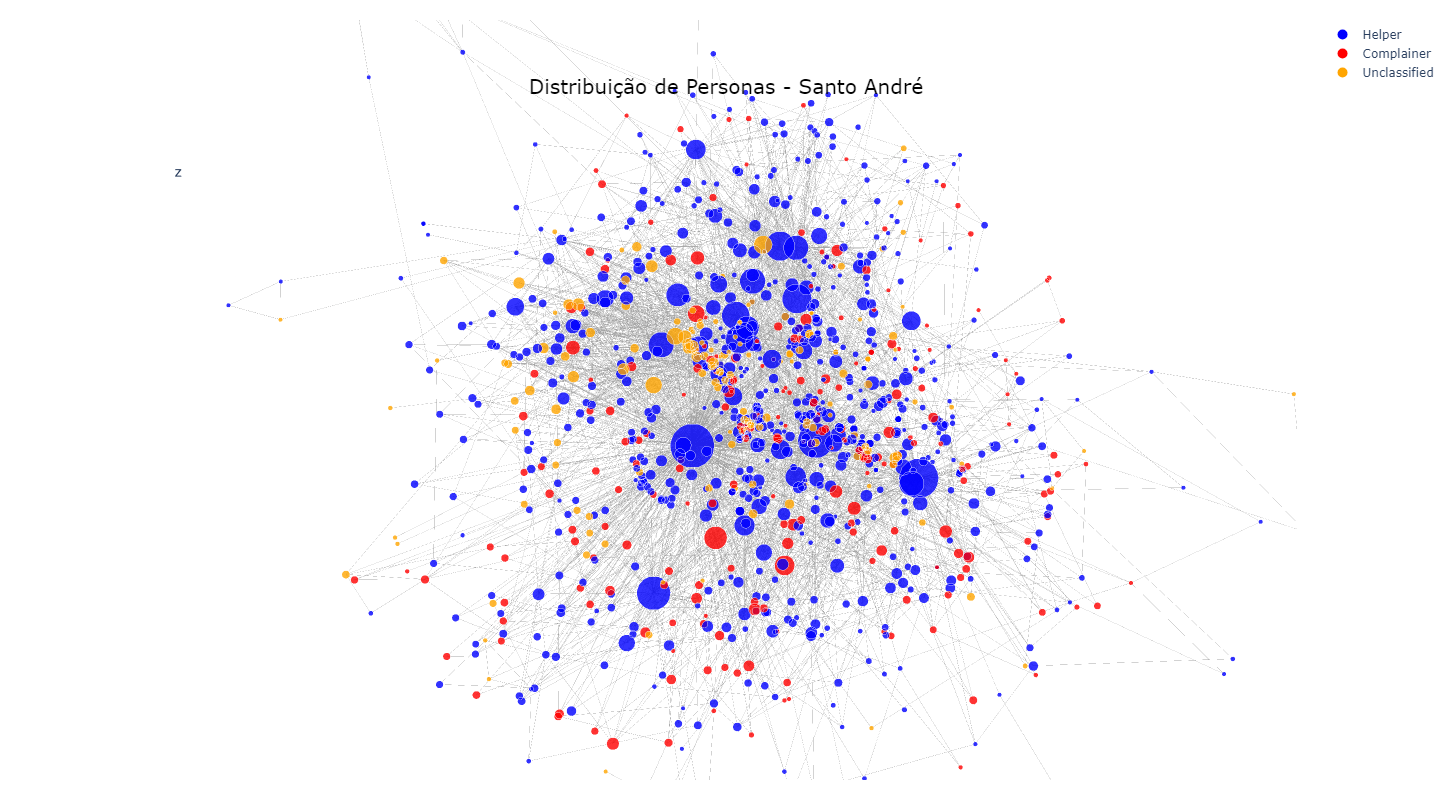
\includegraphics[width=1\textwidth]{images/network_personas_sandre.png}
    \caption{Distribuição de personas na rede de usuários de Santo André.}
    \label{fig:network_personas_sandre}
\end{figure}

Ao observar as métricas de centralidade, notamos que, em média, os \textit{helpers} apresentam graus de entrada e saída mais altos e uma maior centralidade de eigenvector em comparação com os \textit{complainers} em todas as cidades. Este padrão sugere que os \textit{helpers} podem ocupar posições mais centrais e influentes na rede, atuando como hubs de informação e interação. A influência elevada dos \textit{helpers} pode ser um fator determinante na modulação do ambiente online, direcionando o tom e o conteúdo das discussões.

A modulação, medida que indica a estrutura de comunidade bem definida, varia entre as cidades, sendo mais alta na rede que engloba as três cidades e mais baixa em Mesquita. Esta variação pode ser interpretada como uma diferença na coesão das comunidades e na forma como os usuários interagem entre si. Cidades com modulação mais alta podem apresentar comunidades mais isoladas, o que pode favorecer a formação de câmaras de eco.

A matriz de correlação entre as métricas de centralidade e o valor da persona revela relações interessantes. Em todas as cidades, observa-se uma correlação positiva entre o grau de entrada e o grau de saída, bem como entre o grau de entrada e a centralidade de eigenvector. No entanto, a correlação entre o valor da persona e as métricas de centralidade é, em geral, negativa, sugerindo que os \textit{complainers} podem ter uma tendência a ser menos centrais e influentes na rede.

\begin{figure}[h]
    \centering
    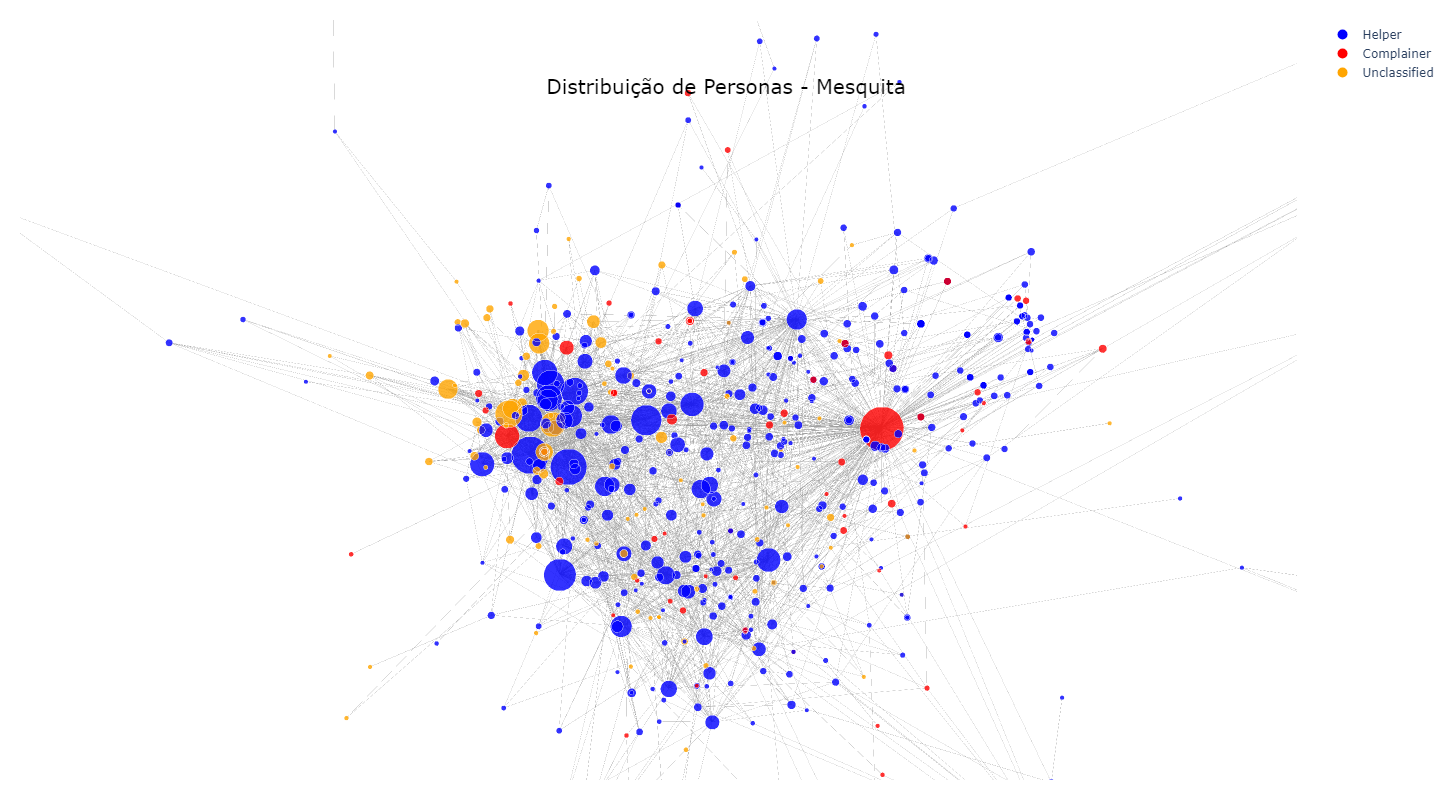
\includegraphics[width=1\textwidth]{images/network_personas_mesquita.png}
    \caption{Distribuição de personas na rede de usuários de Mesquita.}
    \label{fig:network_personas_mesquita}
\end{figure}

A diversidade na estrutura de comunidades, evidenciada pelo número e tamanho das comunidades em cada cidade, sugere diferentes dinâmicas de agrupamento. Mesquita, por exemplo, apresenta o maior número de comunidades, mas com um tamanho médio menor, indicando uma possível fragmentação dos usuários em grupos menores. Esta fragmentação pode ser um terreno fértil para a formação de câmaras de eco, onde opiniões e informações são reforçadas dentro de grupos homogêneos.

Ao considerar o contexto acadêmico, é imperativo refletir sobre como essas descobertas podem contribuir para o entendimento das dinâmicas de interação online e a formação de câmaras de eco. A predominância de \textit{helpers} e sua posição central nas redes podem ser vistas como um mecanismo de resistência contra a polarização e a formação de câmaras de eco, promovendo a diversidade de opiniões e a interação construtiva.

No entanto, a presença de assortatividade positiva e a variação na estrutura de comunidades apontam para a necessidade de estratégias de intervenção e moderação para prevenir a formação de ambientes isolados e polarizados. A compreensão dessas dinâmicas é fundamental para o desenvolvimento de heurísticas e ferramentas que possam detectar e mitigar a formação de câmaras de eco, promovendo um ambiente online mais saudável e inclusivo.

Em conclusão, a análise detalhada das métricas de rede nas três cidades revela padrões e tendências que são essenciais para a compreensão das dinâmicas de interação e a identificação de câmaras de eco. A predominância e influência dos \textit{helpers}, a assortatividade positiva, a diversidade de comunidades e as correlações entre métricas de centralidade e valor de persona são elementos chave que podem guiar futuras pesquisas e intervenções na busca por um ambiente online mais equilibrado e representativo.

A jornada até aqui foi marcada por uma série de experimentos meticulosos, todos com um objetivo comum: construir heurísticas robustas para a detecção de câmaras de eco na rede do Colab. Através da aplicação do modelo de classificação, conseguimos uma visão detalhada das personas dos usuários, revelando nuances sobre como eles interagem e se expressam na plataforma. Esta análise nos mostrou que, apesar de existirem críticos e insatisfeitos, a maioria dos usuários busca colaborar e contribuir de forma positiva.

Ao integrar essas personas na análise de redes, conseguimos ir além da simples classificação. Observamos como as personas se manifestam na estrutura da rede, como se conectam e quais posições ocupam. Esta análise nos deu insights valiosos sobre a dinâmica das interações e sobre como diferentes tipos de usuários influenciam e são influenciados dentro da rede.

No entanto, o mais importante é o que fazemos com esses insights. A detecção de câmaras de eco é mais do que um exercício acadêmico; é uma busca para entender como as opiniões são formadas e reforçadas em ambientes digitais. Ao identificar e compreender essas câmaras, temos a oportunidade de promover diálogos mais abertos e inclusivos, onde diferentes vozes são ouvidas e onde a informação circula de forma mais equilibrada. Com os resultados obtidos, estamos um passo mais perto de tornar o Colab, e outras plataformas digitais, espaços mais saudáveis e representativos para todos os seus usuários.

\section{Homofilia e Câmaras de Eco}

\begin{quadro}[htb]
    \centering
    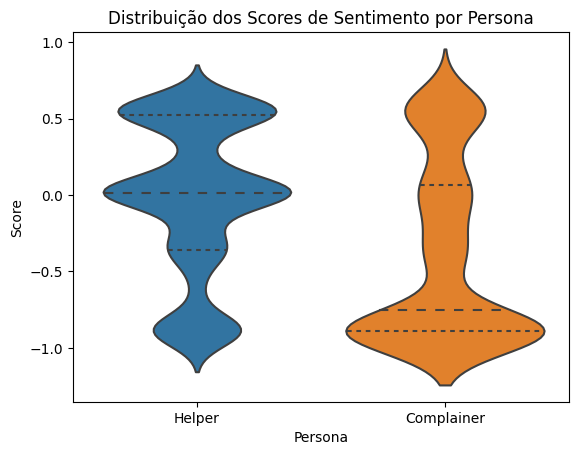
\includegraphics[width=0.8\textwidth]{images/personas_violin.png}
    \caption{Distribuição de Personas por Score (Violin Plot)}
    \label{fig:personas_violin}
\end{quadro}

A homofilia, termo cunhado por Lazarsfeld e Merton em 1954, refere-se à tendência de indivíduos se associarem a outros que são semelhantes a eles em termos de características, interesses e opiniões. Esse fenômeno é amplamente estudado em diversas áreas, incluindo sociologia, psicologia e ciência das redes, e tem sido observado em várias configurações sociais, desde relacionamentos pessoais até interações online em redes sociais.

A homofilia pode estar intimamente relacionada às câmaras de eco, uma vez que a tendência de buscar semelhanças pode levar à formação de grupos com visões e perspectivas convergentes. Quando os indivíduos se associam principalmente a outros que compartilham suas opiniões, informações e conteúdos que são compartilhados dentro desses grupos tendem a reforçar e amplificar essas visões específicas. Isso cria um ambiente propício para o desenvolvimento de câmaras de eco, onde a diversidade de perspectivas é limitada e as ideias divergentes são escassas. A homofilia pode contribuir para a persistência das câmaras de eco ao restringir a exposição a opiniões contrárias e limitar a troca de informações entre diferentes grupos na rede. Essa dinâmica pode resultar em polarização, falta de entendimento mútuo e até mesmo no fortalecimento de crenças extremas.

Estudos têm destacado a relação entre homofilia e câmaras de eco em diferentes contextos, como a propagação de desinformação em redes sociais ou a formação de bolhas de opinião política. A presença de homofilia nas redes sociais pode contribuir para a criação de "filtros de informação" que reforçam as visões existentes e dificultam a exposição a diferentes perspectivas, aumentando assim a probabilidade de formação de câmaras de eco.

Ao entender o conceito de homofilia e sua relação com as câmaras de eco, podemos explorar métricas e técnicas para identificar e mitigar esses fenômenos nas redes sociais. A análise de métricas de homofilia pode fornecer insights sobre a estrutura das redes sociais e ajudar a compreender como as informações são disseminadas e as opiniões são formadas dentro desses contextos específicos. Essas descobertas podem ser fundamentais para desenvolver estratégias e intervenções que promovam uma maior diversidade de perspectivas, diálogo e compreensão mútua na era digital.

As métricas de homofilia geradas a partir deste experimento podem ajudar a detectar câmaras de eco em um grafo da rede do Colab. Câmaras de eco são fenômenos sociais onde as opiniões e informações são amplificadas ou reforçadas pela comunicação e repetição dentro de um sistema fechado e podem contribuir para a polarização social. Ao identificar e entender estas câmaras de eco, podemos desenvolver estratégias para promover a diversidade de opiniões e a comunicação aberta.

\section{Classificação de personas em Modelagem Baseada em Agentes}

A Modelagem Baseada em Agentes (MBA) é uma técnica computacional que tem ganhado interesse em diversas áreas de pesquisa, devido à sua capacidade de simular a interação de agentes autônomos e observar os resultados emergentes dessas interações. A MBA é particularmente útil para estudar sistemas complexos, onde o comportamento global do sistema não pode ser facilmente deduzido a partir do comportamento individual dos agentes.

Agora, consideremos as personas \textit{helpers} e \textit{complainers}. Estas personas, embora não sejam explicitamente mencionadas por Atiqi, podem ser consideradas como agentes dentro da estrutura de MBA. Os \textit{helpers} podem ser vistos como agentes que buscam transmitir mensagens positivas e úteis, enquanto os \textit{complainers} tendem a transmitir mensagens negativas ou críticas. A interação entre essas duas personas pode levar a diferentes dinâmicas de rede e padrões de comunicação. Por exemplo, se os \textit{helpers} são mais influentes ou numerosos, eles podem criar um ambiente mais positivo e cooperativo na rede social. Por outro lado, se os \textit{complainers} são mais influentes ou numerosos, eles podem criar um ambiente mais negativo e crítico. 

Além disso, a presença de bots também pode influenciar a dinâmica entre \textit{helpers} e \textit{complainers}. Por exemplo, bots programados para agir como \textit{helpers} podem aumentar a positividade e a cooperação na rede, enquanto bots programados para agir como \textit{complainers} podem aumentar a negatividade e a crítica. Portanto, a abordagem de MBA usada por Atiqi se torna uma ferramenta útil para estudar a interação entre \textit{helpers} e \textit{complainers} em redes sociais e entender como essas interações podem influenciar a dinâmica da rede e a formação da opinião pública.

Dentro desse contexto, Atiqi introduz o conceito de "opinião média", que pode ser entendido como uma métrica que reflete a tendência geral ou o sentimento dominante em uma rede social em um determinado momento. A opinião média é calculada com base nas postagens e interações dos usuários, e pode ser influenciada tanto por \textit{helpers} quanto por \textit{complainers}, bem como por outros fatores externos, como notícias ou eventos atuais.

A ideia de calcular a opinião média é crucial para entender a dinâmica de uma rede social. Se, por exemplo, a opinião média em uma rede social é predominantemente positiva, isso pode indicar que os \textit{helpers} estão tendo um impacto maior na formação da opinião pública. Por outro lado, uma opinião média predominantemente negativa pode indicar uma influência maior dos \textit{complainers}.

No contexto da plataforma Colab, podemos adaptar essa ideia para extrair a opinião média dos usuários com base em suas postagens. Ao analisar o conteúdo, a frequência e o sentimento das postagens dos usuários, podemos calcular uma opinião média para diferentes tópicos ou áreas de interesse. Por exemplo, se muitos usuários estão postando sobre problemas de transporte público e expressando insatisfação, a opinião média sobre esse tópico seria negativa.

Para criar heurísticas que nos ajudem a extrair essa opinião média, podemos começar categorizando postagens com base em palavras-chave ou tópicos específicos. Em seguida, podemos analisar o sentimento dessas postagens usando técnicas de processamento de linguagem natural. Ao combinar essas informações com os dados de persona dos usuários, podemos obter uma visão mais completa da opinião média em diferentes tópicos.

No próximo capítulo, introduziremos o conceito de barômetro social hiperlocal. Este modelo inovador promete revolucionar a forma como interpretamos e analisamos as dinâmicas de redes sociais como o Colab. Exploraremos em detalhes como esse barômetro pode ser utilizado para calcular a opinião média dos usuários, levando em consideração tanto o sentimento expresso em suas postagens quanto as personas associadas a cada um. Além disso, discutiremos como a combinação de técnicas de processamento de linguagem natural e Modelagem Baseada em Agentes pode proporcionar insights mais profundos sobre a formação da opinião pública e a dinâmica de interação entre diferentes grupos de usuários. Através dessa abordagem, buscamos não apenas entender, mas também prever tendências e padrões de comportamento dentro da plataforma, permitindo uma resposta mais eficaz e informada a diferentes cenários e desafios.